\chapter{System Architektur}
\label{kap:Kapitel03}

\section{Überblick}
Im folgenden wird nun die System Architektur und der Workflow erläutert, welche als Grundlage für die Studie dienten, um die in 1.2 geschilderte Problemstellung abzubilden und letztendlich zu lösen.

\subsection{Architektur}
\label{subsec:architecture}
Um ein besseres Bild davon zu bekommen, wie die einzelnen Komponenten
zusammenhängen bzw. welche Aufgaben diese in Wechselwirkung zu anderen Instanzen übernehmen und ausführen, wird zunächst die Architektur des Systems erläutert. Als Basis soll dabei die Abbildung \ref{img:abb2} dienen, anhand jener vorrangig die jeweiligen Komponenten bezüglich ihrer Funktionsweise beschrieben werden. Das Zusammenspiel der Anwendungen wird im Anschluss unter \ref{subsec:workflow} detailliert beleuchtet.

\clearpage
\newpage

\begin{figure}[th!]
	\centering
	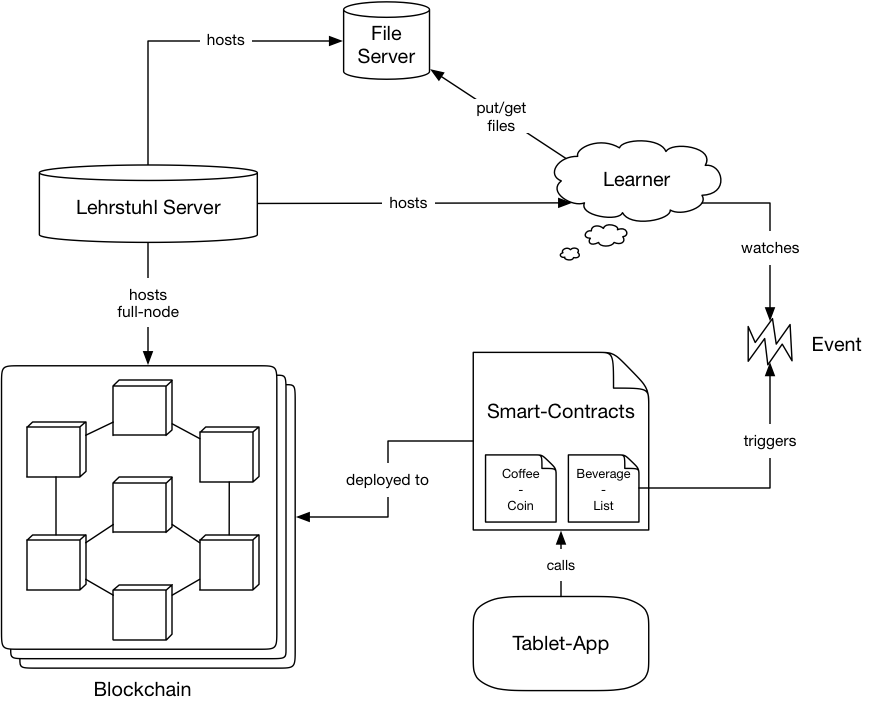
\includegraphics[width=.99\columnwidth]{./Abbildungen/Kapitel_03/system_architecture.png}
	\caption{Systemarchitektur}
	\label{img:abb1}
\end{figure}
\FloatBarrier

\nlparagraph{Lehrstuhl Server}
Der Lehrstuhlserver ist dafür zuständig einen Großteil der Anwendungen zu hosten bzw. zu starten.
Dies gilt sowohl für den HTTP-Fileserver als auch für die Learner-Anwendung, welche dessen Betriebssystem als Plattform nutzen.\\
Auch die Blockchain wird auf dem Server gestartet und verwendet diesen zudem als full-node, um Transaktionen zu minen.
Der Server ist im Grunde der Anwendungen, dessen primäre Funktionsweise darin besteht jenen eine Plattform zu bieten und mit Rechenleistung zu versorgen.

\nlparagraph{Learner}
Der sogenannte \quotes{Learner} ist eine in Golang implementierte Softwareanwendung, dessen Hauptaufgabe darin besteht, das Kaffeetrinkverhalten der Nutzer zu erlernen - wovon auch die Namensgebung der Anwendung stammt.
Um dies zu erreichen, wurde die Anwendung in Submodule unterteilt, welche einen dedizierten Aufgabenbereich abdecken und diesen eigenständig bearbeiten.
Auch wenn jene für sich autark agieren können, kann das Trinkverhalten letztendlich erst in der gegenseitigen Wechselwirkung jener erlernt werden. \\
Die Submodule lauten wie folgt:
\begin{itemize}
	\item Q-Learning
	\item Worker
	\item Watcher
	\item (Smart Contract Deployment Skript)
\end{itemize}

Das \textbf{Q-Learning} ist, wie der Name bereits impliziert, für das eigentliche Erlernen des Trinkverhaltens zuständig. Es ist im Grunde die Implementierung des Q-Learning Algorithmus, sowie die damit einhergehende Zustandsraummodiellerung, welches aber unter ref{subsec:ql} genauer erläutert wird.
\\\\
Der \textbf{Worker} ist einerseits für die Userverwaltung und andererseits für die, in einem festgelegten Intervall, Ausführung des Q-Learning Algorithmus, zuständig. (vgl. Kap. \ref{subsec:learning})
\\\\
Der \textbf{Watcher} beobachtet Events, die vom Smart-Contract \quotes{Beveragelist} ausgelöst wurden. Die Daten, welches das Event beinhaltet, werden daraufhin verwendet um den Q-Learning Algorithmus zu befüllen und aufgrund diesen das Trinkverhalten zu erlernen.
\\\\
Das \textbf{Smart Contract Deployment Skript}, ist in der Form zwar nicht in der Systemarchitektur vorhanden, da es aber auch ein Submodul des Learners und für das gesamte Konstrukt dahingehend essentiell ist, da es die Smart Contracts auf der Blockchain installiert und im Zuge dessen erst die Verbindung zwischen Blockchain und Learner ermöglicht, wird es in dieser Auflistung trotzdem aufgeführt.

\nlparagraph{Fileserver}
Der Fileserver ist eine Go-Anwendung, welche eine rudimentäre REST \cite{REST:Wiki} Api \cite{API:Wiki} zur Verfügung stellt.
Von den sogenannten CRUD \cite{CRUD:Wiki} Operationen, welche als grundlegend für alle persistenten Datenspeicher angesehen werden können, implementiert dieser nur das \quotes{GET} und das \quotes{PUT}. Sowohl die \quotes{PATCH} als auch die \quotes{DELETE} Operation bieten keinen Mehrwert für die Gesamtarchitektur bzw. den Workflow und sind in Anbetracht dessen nicht implementiert.\\
Das bedeutet die Hauptaufgabe des Fileservers besteht darin, Dateien zu empfangen und zu speichern (PUT) und diese auf Anfrage (GET) an einen Antragsteller wieder zu versenden.\\
Außerdem bietet die Anwendung zusätzlich zur Api einen UDP-Broadcast, welcher v.a. beim Testing und beim Setup eine große Erleichterung darstellt. Dieser Broadcast versendet in seinen Nachrichten lediglich die IP-Adresse des Lehrstuhl-Servers und somit auch seine eigene und die der Blockchain.
Da die IP-Adresse und der Port des Broadcasts stets gleich bleiben, sich aber die Host-IP der Blockchain und des Fileservers je nach Deployment theoretisch ändern können - was in der Entwicklungsphase sehr oft der Fall war. Müssen sich sowohl der Learner als auch die Tablet-App lediglich auf den Broadcast \quotes{subscriben} und können dadurch die IP der Blockchain und des Fileservers erfahren. Durch diese dynamische Zuweisung der IP-Adresse, müssen keine Updates beim Learner und der App durchgeführt werden, sollte die Blockchain und der Fileserver auf einem anderen Host deployed werden. \\
Aufgrund der Tatsache, dass sich die IP-Adresse des Lehrstuhl-Servers während der Studie nicht ändert, ist der UDP-Broadcast auch nicht in der Abbildung \ref{img:abb1} der Systemarchitektur berücksichtigt worden. Der Anwendungsbereich ist trotz alledem im Bereich der Testphase und auch für die künftige Projekte,bei denen das System Verwendung findet, definitiv vorhanden.

\clearpage
\nlparagraph{Blockchain}
Die Blockchain ist eine private, eigens für die Studie erstellte Ethereum-Blockchain, dessen \quotes{Genesis-Block} aus dem JSON-File (vgl. Abbildung \ref{img:abb3}) generiert wird. Die Erläuterungen zu den jeweiligen Key-Value-Pairs sind unter Kap. \ref{subsec:genesis} zu finden.
Das Generieren und das Starten der Blockchain erfolgt auf dem Lehrstuhlserver.
Dabei hostet der Server zudem eine sogenannte \quotes{full-node} (auch \quotes{miner} genannt) der Blockchain, welche dafür zuständig ist Transaktionen zu berechnen und zu bestätigen.
Aus Ressourcengründen ist dieser \quotes{miner} der einzige im Gesamtsystem, was aus theoretischer Sicht einen \quotes{Single Point of Failure} \cite{SPOF:Wiki} als Nachteil mit sich zieht. Das bedeutet sollte diese \quotes{full-node} ausfallen, würden keine Transaktionen mehr bestätigt werden. Da es weder während der Entwicklungsphase noch während der Studie zu einem einzigen Ausfall kam, ist dieser Nachteil als sehr klein einzuschätzen, weswegen auch keine weitere \quotes{full-node} zum System hinzugefügt wurde. Der große Vorteil besteht allerdings darin, dass Transaktionen sehr schnell bestätigt werden, da es keine weiteren \quotes{node's} gibt, die um die Berechnung eines Block's konkurrieren. Was vor allem aus Sicht der User-Experience \cite{UE:Wiki} einen großen Mehrwert darstellt, da dieser in wenigen Sekunden erfährt, ob seine Transaktion erfolgreich durchgeführt wurde. Dies kann bei anderen Blockchains wie z.B. Bitcoin bis zu 10 Minuten dauern \cite{MINING:kryptopedia}, was im Kontext der Systemarchitektur nicht tragbar wäre.\\\\
Um letztendlich mit der Blockchain kommunizieren und dessen Potential in voller Gänze ausschöpfen zu können, werden auf diese sogenannte Smart-Contracts \cite{SC:EconomyOutlook} deployed. Im Rahmen der Systemarchitektur sind es zwei dedizierte Smart-Contracts (\textit{Coffe-Coin}, \textit{Beverage-List}), welche komplett unabhängig voneinander agieren.

\clearpage
\nlparagraph{Smart Contracts}
Die beiden Smart Contracts welche auf die Blockchain deployed werden, werden mit \textit{Coffe-Coin} und \textit{Beverage-List} betitelt.
Diese decken zwei völlig unterschiedliche Aufgabenbereiche ab, weswegen sie keinen Einfluss aufeinander haben und deswegen unabhängig voneinander operieren.
So löst nur der \textit{Beverage-List Contract} ein Event aus, sobald eine bestimmte Funktion dessen aufgerufen wird. \\
Die Ausführung (\textit{call}) beider erfolgt jedoch stets von Seiten der \textit{Tablet-App}. Diese ist auch die einzige Instanz, welche in Form von Transaktionen mit der Blockchain interagiert.

\nlparagraph{Tablet-App}
Die \textit{Tablet-App} ist eine mit React-Native \cite{RN:ReactNative} erstellte Crossplattform App \cite{CP:Wiki}, welche auf einem Android Tablet installiert ist. Die Hauptaufgabe der App ist es Funktionen der beiden Smart Contracts aufzurufen, in dem es die benötigten Daten an den Smart Contract übergibt, um schlussendlich Transaktionen auszulösen.\\
Damit eine Kommunikation mit einem Smart Contract überhaupt zustande kommt, schickt die App einen Request an den Fileserver, welcher mit den angefragten Smart Contract Daten in Form einer Datei antwortet.
\nlparagraph{Event}
Das Event beschreibt im Grunde die indirekte Kommunikation zwischen dem \textit{Learner} und der \textit{Tablet-App} mit dem Smart Contract \textit{Beverage-List} als Mittelsmann. So wird jenes im Zuge eines Funktionsaufrufs des Smart Contracts von Seiten der App ausgelöst und vom \textit{Learner} detektiert und der Inhalt zum Erlernen des Kaffeetrinkverhaltens verwendet.
\clearpage

\subsection{Workflow}
\label{subsec:workflow}
Die unter Kap. \ref{subsec:architecture} beschriebene Architektur wird im folgenden unter dem Gesichtspunkt des Workflows, also dem Zusammenspiel der einzelnen Komponenten und dem Gesamtablauf, näher betrachtet. Dabei beschreibt der Gesamtablauf die einzelnen Schritte startend beim Setup der Komponenten hin zum eigentlichen Durchlauf der einzelnen Softwareanwendungen, was letztlich im Erlernen des Kaffeetrinkverhaltens resultiert. Im Zuge dessen werden auch einzelne Algorithmen der Instanzen und Kommandos kurz erläutert, um ein besseres Verständnis für die Funktionsweise der Anwendungen zu bekommen. \\\\
Der Workflow lässt sich in zwei Phasen unterteilen. In der ersten werden die einzelnen Komponenten konfiguriert und gestartet und die zweite beschreibt den eigentlichen Ablauf und das Zusammenwirken der Instanzen.

\paragraph{Setup}
\begin{legal}
	\item {Blockchain}
	\begin{legal}
		\item erstellen \& konfigurieren
		\item starten
	\end{legal}
				      	       	                            
	\item Fileserver
	\begin{legal}
		\item REST Api starten
		\item UDP Broadcast starten
	\end{legal}
				      	       	                            
	\item Smart Contracts
	\begin{legal}
		\item deploy Beveragelist Smart Contract und sende JSON-File mit ABI und Adresse an Fileserver
		\item deploy CoffeeCoin Smart Contract und sende JSON-File mit ABI und Adresse an Fileserver
	\end{legal}
				      	       	                            
	\item Learner
	\begin{legal}
		\item Worker starten
		\item Watcher starten
	\end{legal}
				      	       	                            
	\item Tablet App
	\begin{legal}
		\item installieren
		\item starten
	\end{legal}
				      	       	                                
\end{legal}

Die Punkte 1. und 2. sowie 4. und 5. können auch parallel ausgeführt bzw. deren Reihenfolge vertauscht werden.\\\\
Im ersten Schritt muss die private Blockchain erstellt werden. Dabei müssen zuerst die benötigten Accounts generiert und daraufhin die Blockchain erzeugt werden. Sollte 1a) zu einem früheren Zeitpunkt bereits durchgeführt worden sein, kann dieser Punkt übersprungen und gleich mit 1b) begonnen werden.
Sobald 1a) einmal durchgeführt wurde, kann die Blockchain gestartet werden.
\\\\ Dies geschieht mit folgendem Befehl:\\

\newlength{\imageheight}
\settoheight{\imageheight}{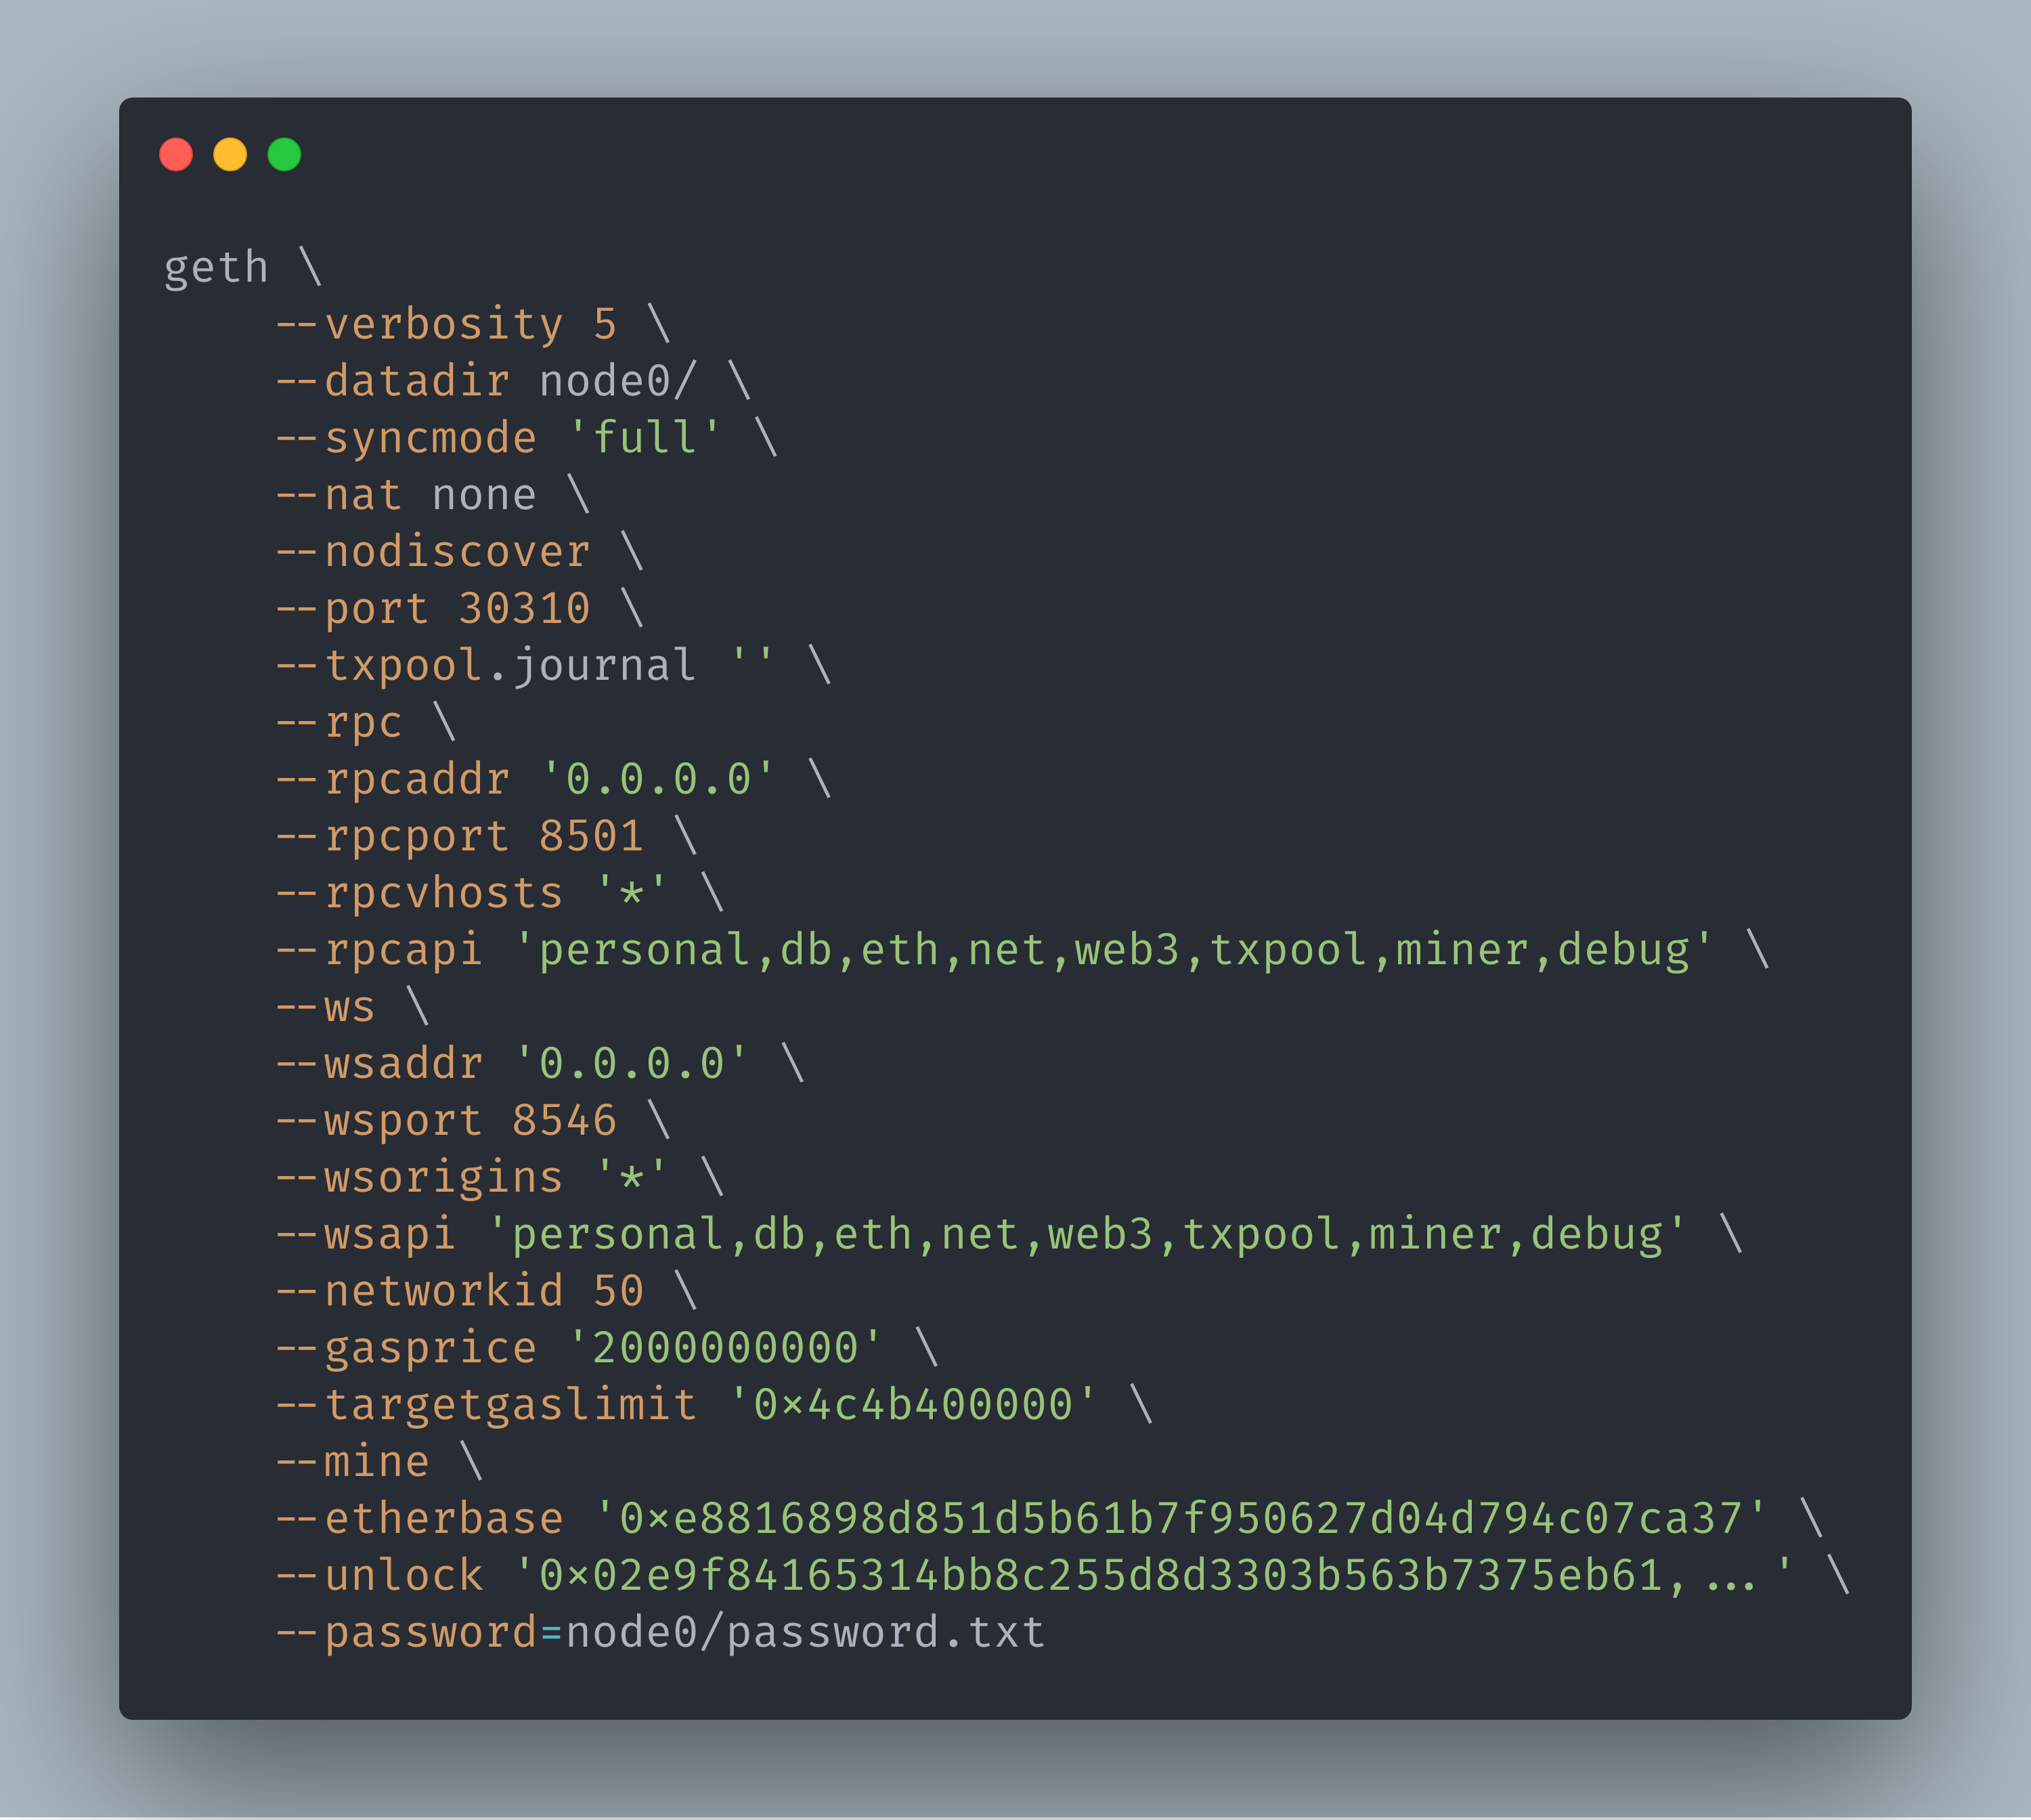
\includegraphics{./Abbildungen/Kapitel_03/geth.png}}
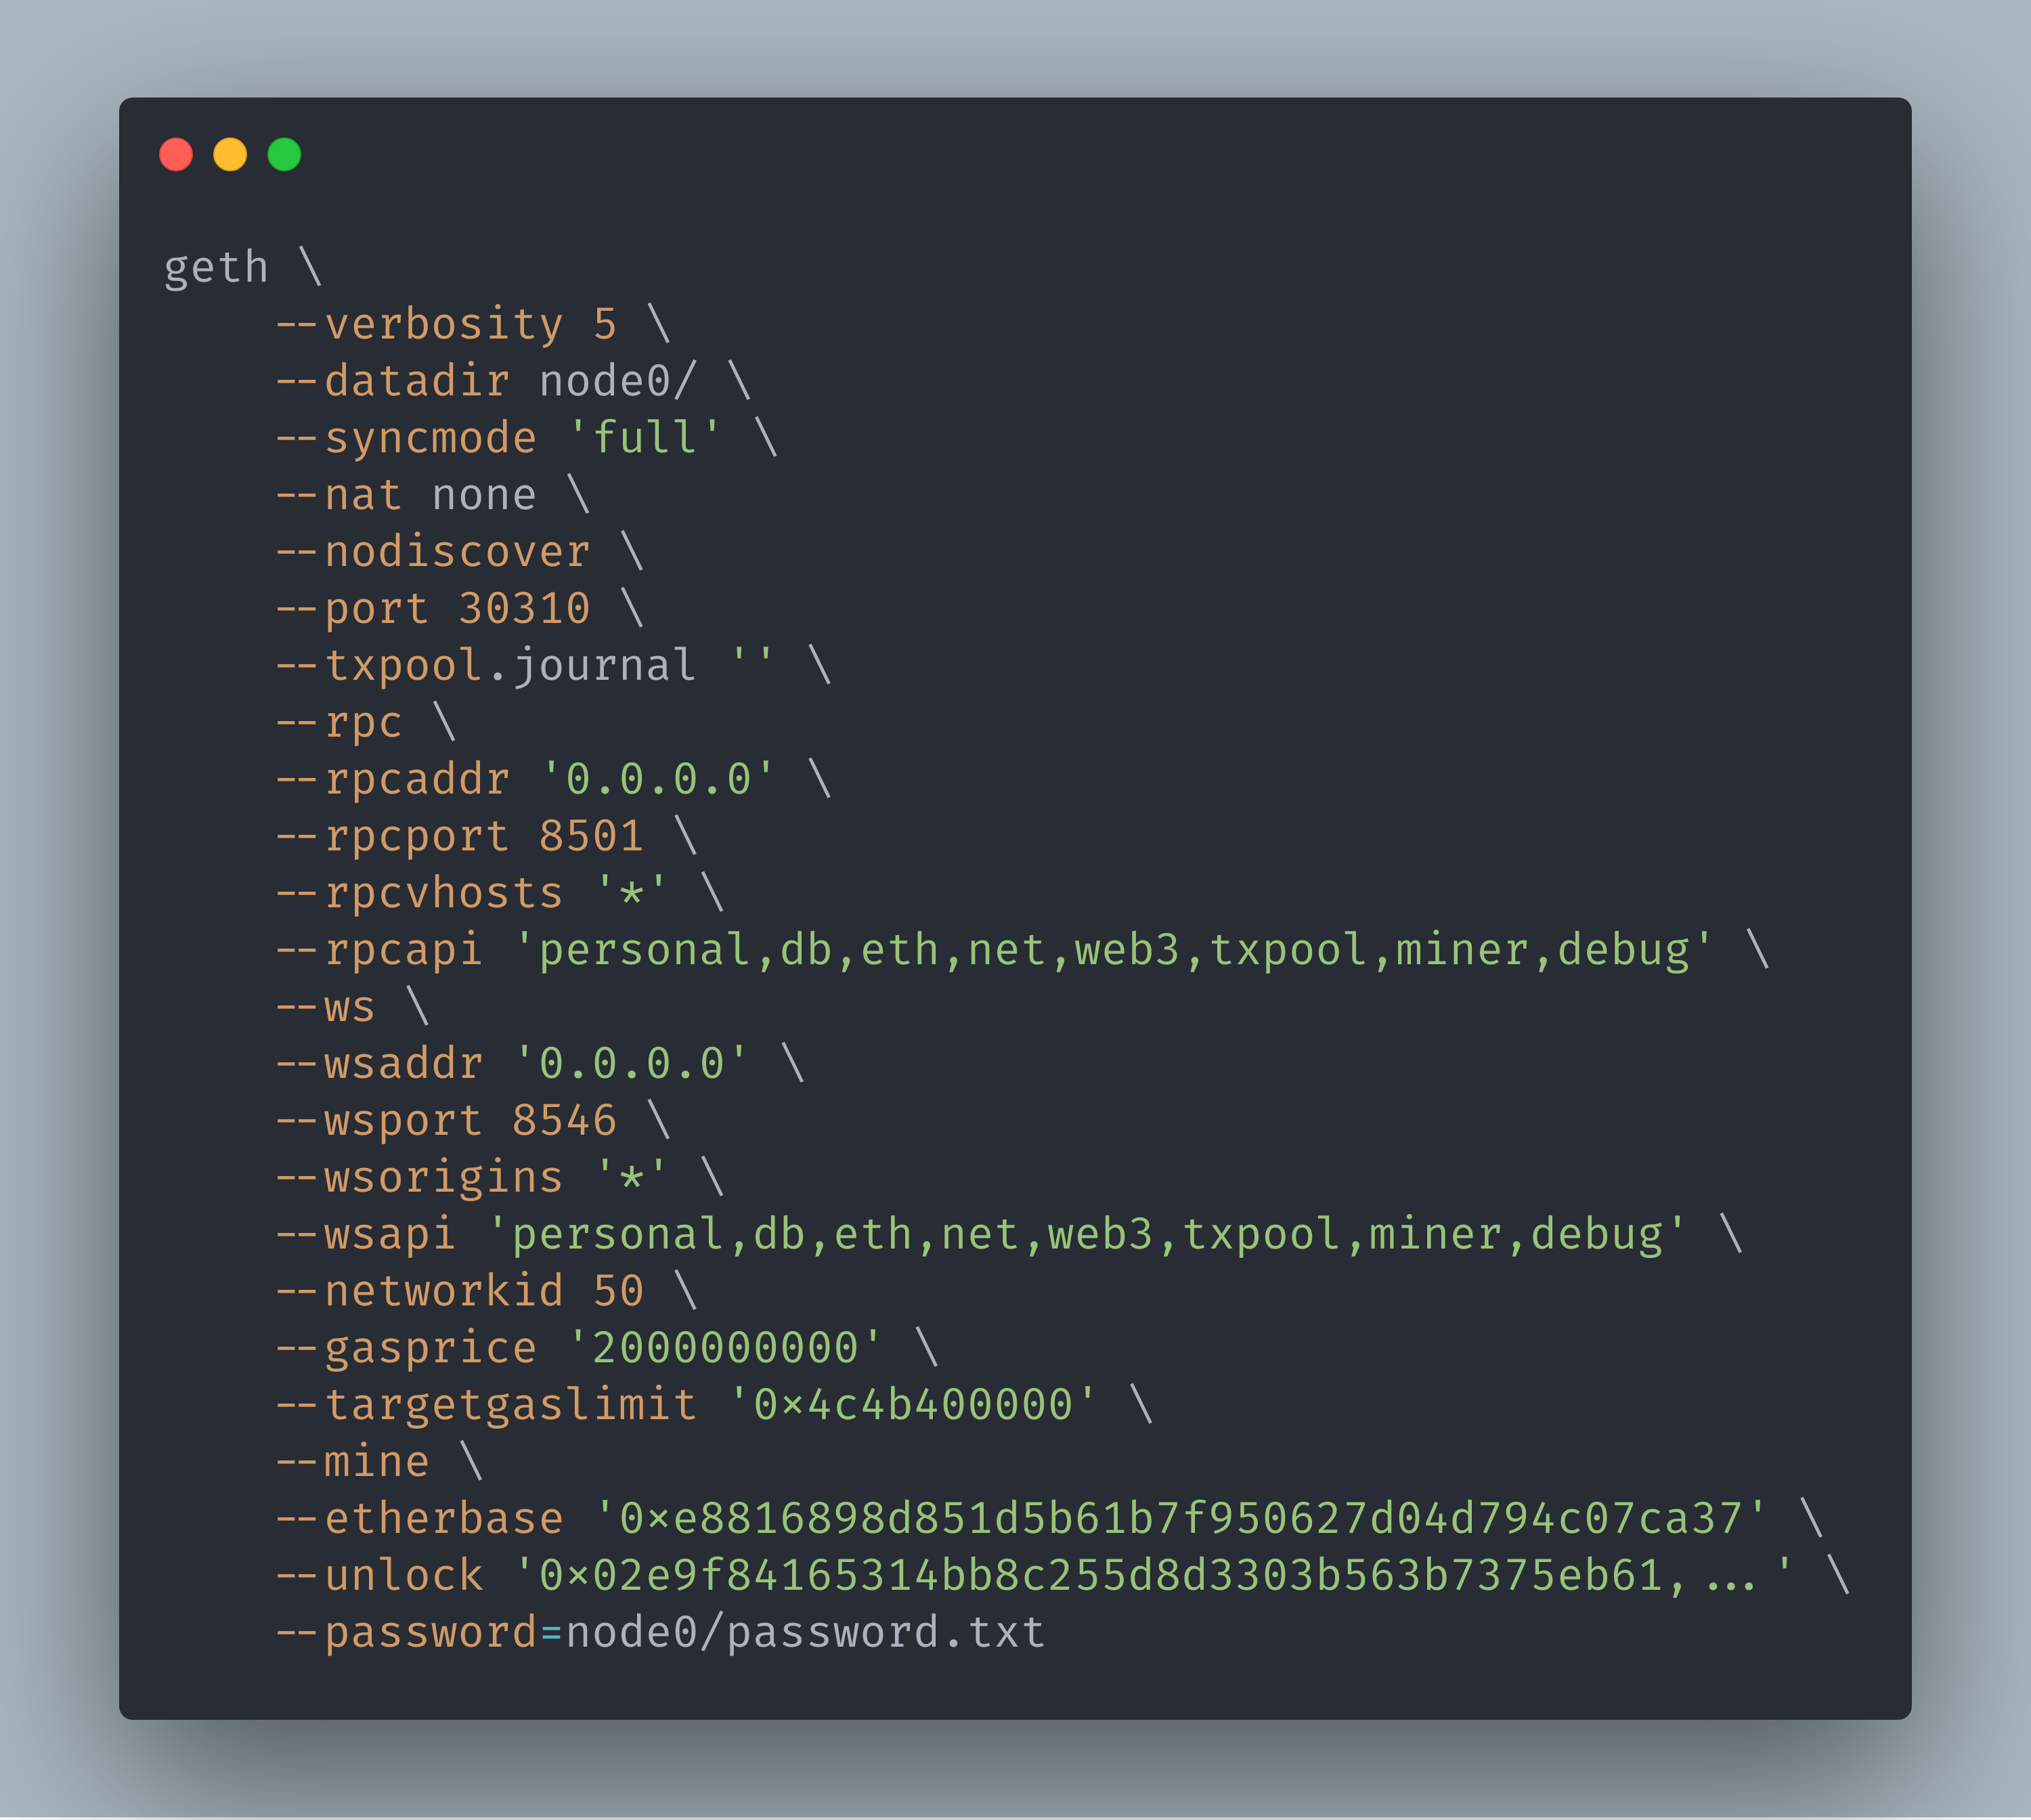
\includegraphics[trim=0 0.49\imageheight{} 0 0, clip, width=.9\columnwidth]{./Abbildungen/Kapitel_03/geth.png}

\clearpage

\begin{figure}[hbt!]
	\centering
	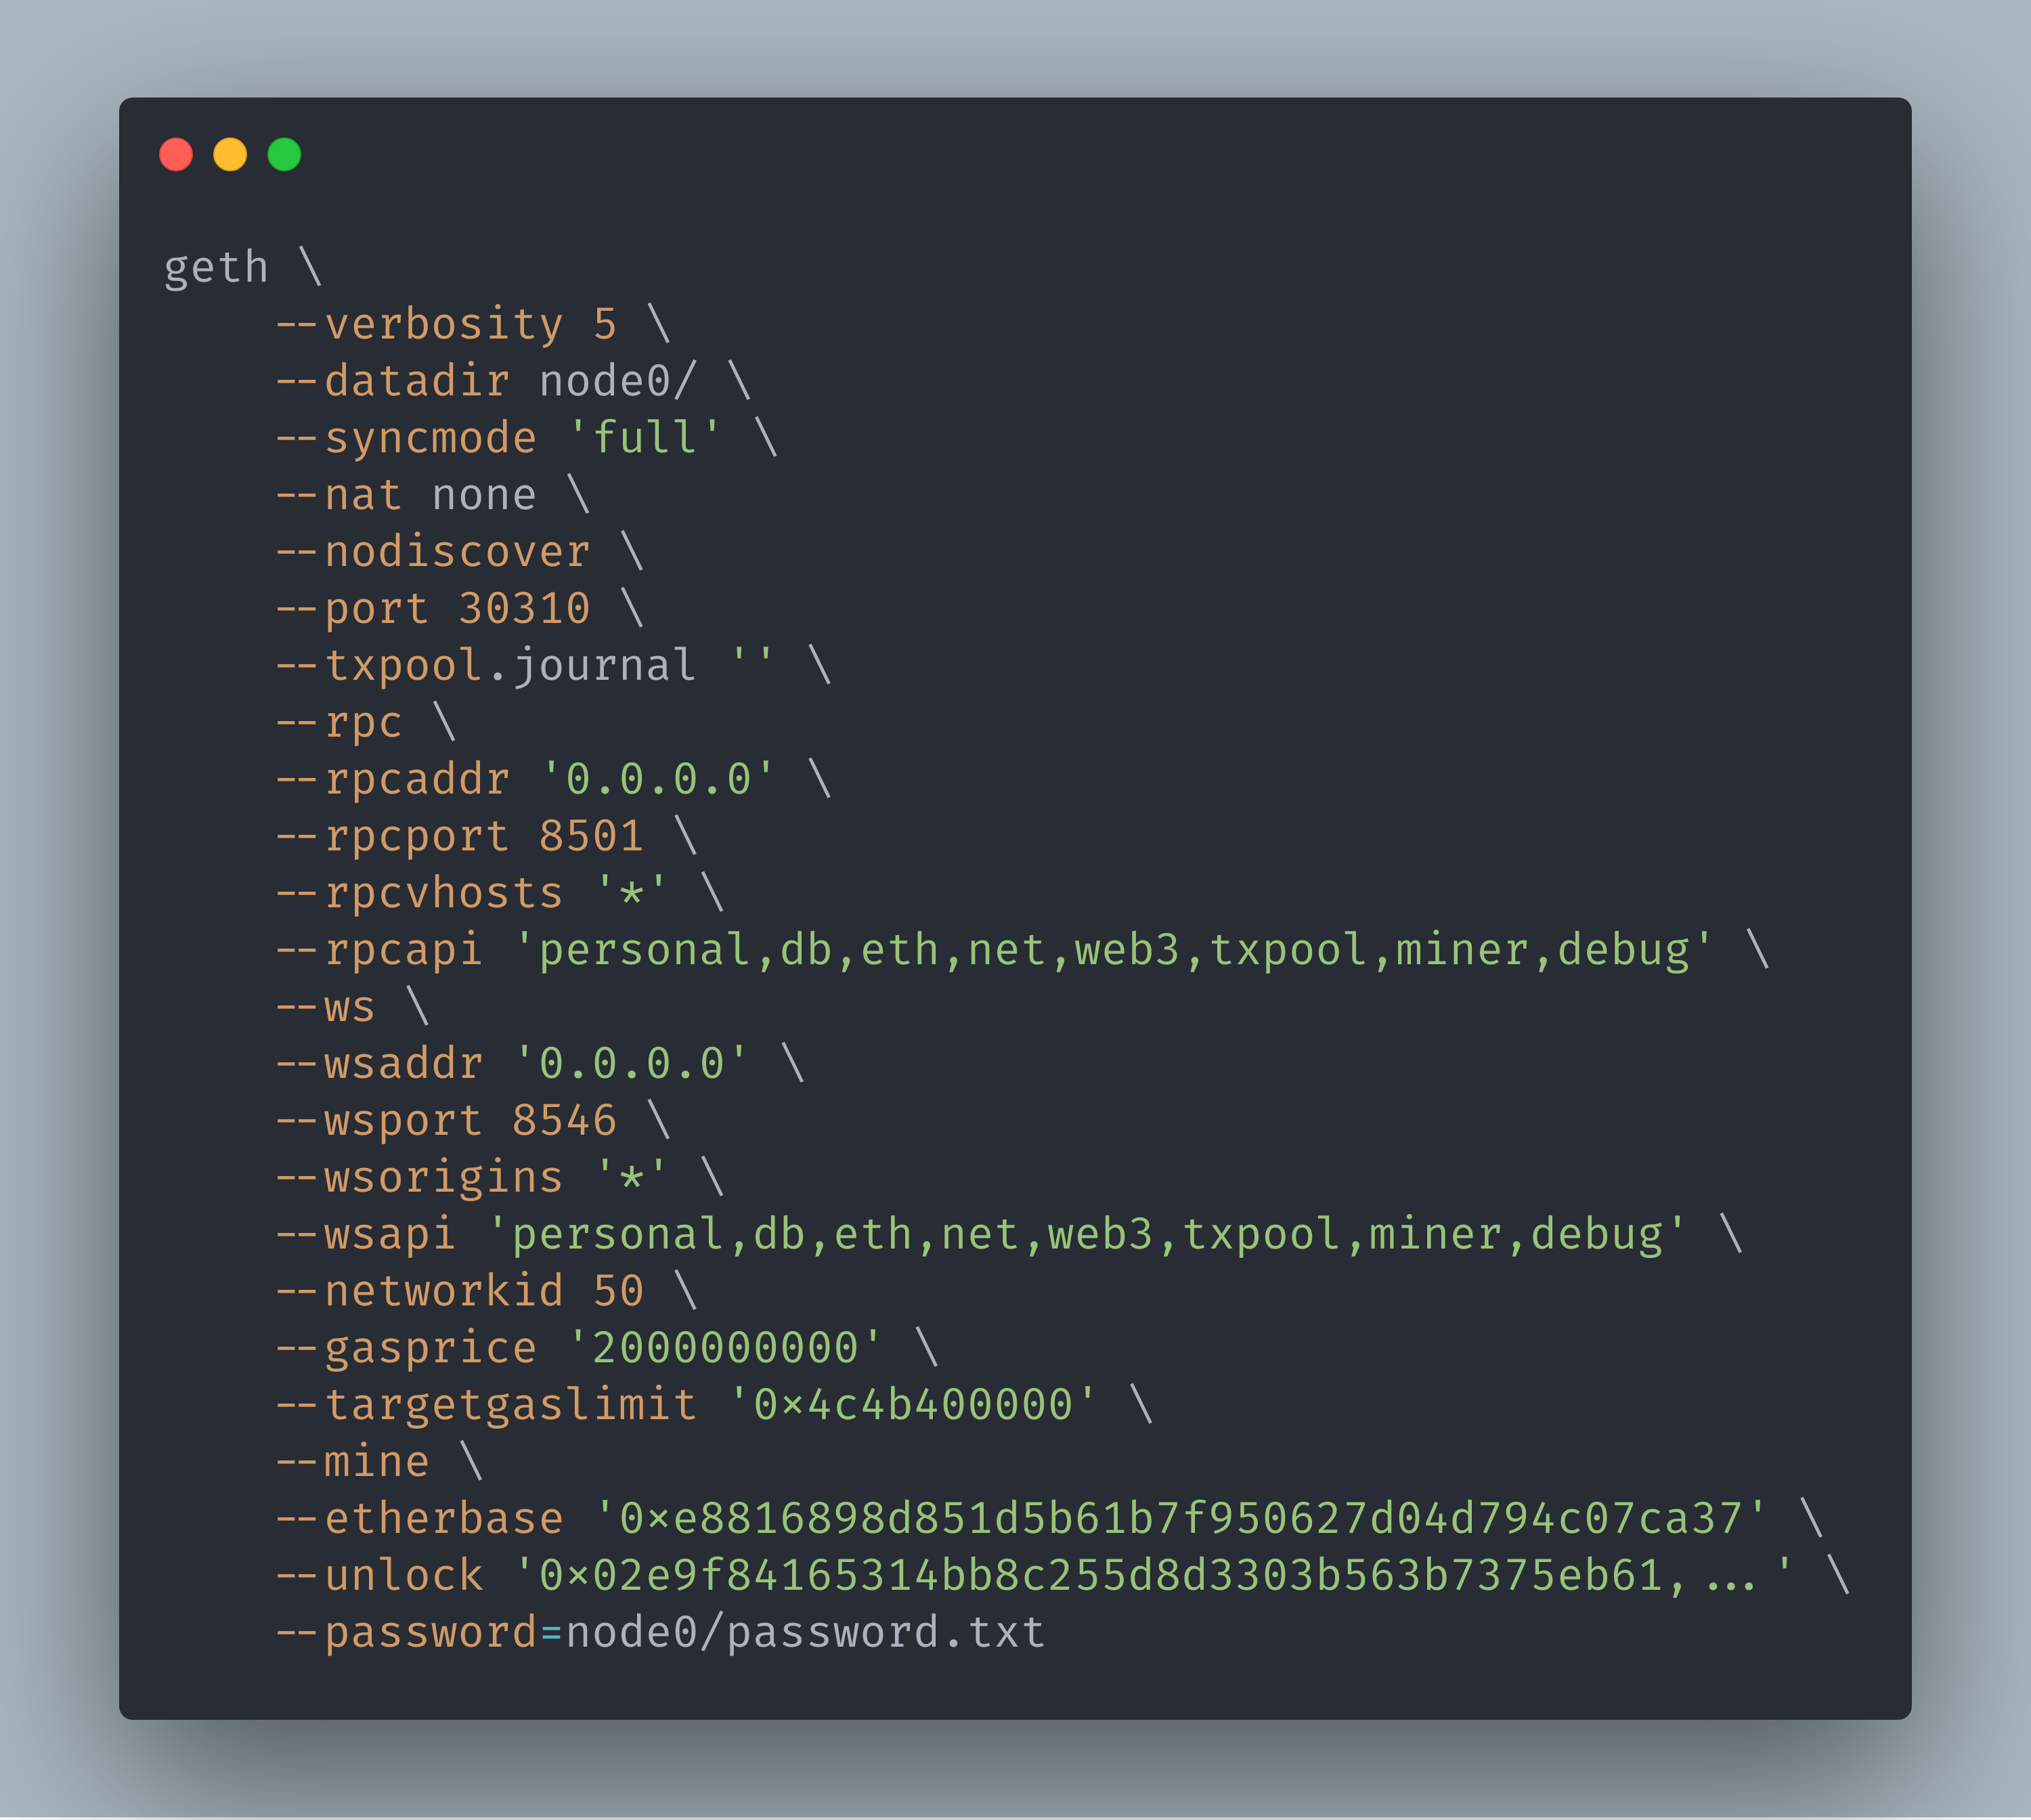
\includegraphics[trim=0 0 0 0.503\imageheight{}, clip, width=.9\columnwidth]{./Abbildungen/Kapitel_03/geth.png}
	\caption{geth Befehl zum starten der Blockchain}
	\label{img:geth}
\end{figure}

Dieser Befehl setzt zum einen weitere Konfigurationsparameter der Blockchain. So wird z.B. festgelegt unter welcher IP-Adresse und Port (\textit{-{}-rpcaddr}, \textit{-{}-rpcport}, \textit{-{}-wscaddr}, \textit{-{}-wsport}) die Blockchain erreichbar ist und welche Api-Befehle unter dieser Schnittstelle ausgeführt werden dürfen (\textit{-{}-rpcapi}, \textit{-{}-wsapi}). \\
Zum anderen wird aber zugleich auch eine sogenannte \textit{full node} gestartet (\textit{-{}-syncmode}), die durch das \quotes{Flag} \textit{-{}-mine} sofort zum \quotes{minen} beginnt.\\
Desweiteren werden alle Accounts entsperrt die unter (\textit{-{}-unlock}) gelistet sind und deren Passwörter in der angegebenen Textdatei bei (\textit{-{}-password}) hinterlegt sind. \\\\
Damit eine \textit{Node} Daten speichern kann, muss ein Verzeichnis angegeben werden (\textit{-{}-datadir}), in dem Dateien abgelegt werden können. Hier werden z.B. die Daten der Accounts oder auch die Textdatei mit den Passwörtern (\textit{-{}-password}) gespeichert.\\\\
Wurde die Blockchain in Betrieb genommen, wird im nächsten Schritt die REST Api und der UDP Broadcast des Fileservers gestartet. \\
Daraufhin ist es möglich die beiden Smart Contracts zu deployen. Dabei wird jeweils für 3a) und 3b) das identische Bash-Skript mit unterschiedlichen Eingabeparametern ausgeführt. Dieses Skript liest zuerst die Datei des angegebenen Smart Contracts ein und erzeugt daraufhin die Binaries und die ABI,
welche schlussendlich dazu verwendet werden ein Go Bindingsfile zu generieren.
Im Anschluss wird dann ein Go-Skript ausgeführt, welches auf Grundlage des Bindingsfiles den Smart Contract auf der Blockchain installiert und die zurückgelieferte Adresse und die bereits bekannte ABI ein JSON-File packt und an den Fileserver schickt.\\\\
Wurden die Smart-Contracts erfolgreich deployed, kann der Learner gestartet werden. Dieser \quotes{subscribed} sich im ersten Schritt auf den UDP Broadcast und extrahiert aus den Nachrichten die IP-Adresse der Blockchain und des Fileservers. Daraufhin werden sowohl der Worker als auch der Watcher in Form von \quotes{Goroutines} aktiviert. Der Worker iteriert über die Liste aller User und kontaktiert jeweils den Fileserver ob bereits gelernte Daten für diesen Usern vorhanden sind. Sollte das Fall sein, initialisiert er damit die Parameter des Q-Learning Algorithmus des Users.\\
Der Watcher schickt ebenfalls eine Anfrage an den Fileserver und bekommt als Antwort die Daten der Smart Contracts. Daraufhin kann er sich mit der Blockchain verbinden und sich auf die Events des Beveragelist Smart Contracts \quotes{subscriben}.\\\\
Abschließend wird die App auf dem Tablet installiert, sollte sich diese noch nicht auf dem Tablet befinden und daraufhin gestartet. Die Initialisierung erfolgt hierbei nach dem selben Prinzip wie beim Learner. Zuerst wird der UDP Broadcast nach der Server Adresse abgefragt, mit welcher anschließend der Request an den Fileserver geschickt wird, um die benötigten Smart Contract Daten zu bekommen. Welche im Anschluss dazu verwendet werden eine Verbindung zur Blockchain bzw. zu den Smart Contracts herzustellen.
\\\\
Erfolgte eine fehlerlose Abarbeitung dieser Schritte, kann zum eigentlichen Workflow übergegangen werden.
\clearpage
\paragraph{Workflow}
\begin{legal}
	\item {App}
	\begin{legal}
		\item User wählt Getränk aus
		\item \textit{call} CoffeeCoin
		\item \textit{call} Beveragelist
	\end{legal}
				      	       	                            
	\item Smart Contracts
	\begin{legal}
		\item Beveragelist \textit{triggers} Event
	\end{legal}
				      	       	                              
	\item Learner
	\begin{legal}
		\item Watcher:
		\begin{legal}
			\item detektiert Event
			\item extrahiert Daten aus Event
			\item befüllt Q-Learning Algorithmus mit den Event-Daten (evaluate \& predict)
		\end{legal}
		\item Worker (periodisch alle 3h)
		\begin{legal}
			\item \quotes{triggers} Q-Learning Algorithmus (evaluate \& predict)
			\item sendet gelernte Daten (vgl. Abbildung \ref{img:abb2}) an Fileserver
		\end{legal}
	\end{legal}
\end{legal}

Diese Auflistung beschreibt einen synchronen, erfolgreichen Durchlauf der Systemarchitektur - die Asynchronität des Workers 3b) außer Acht gelassen. Alternative Abläufe sowie Zustände die aus Fehlern resultieren, werden bei den einzelnen Komponenten nochmals genauer betrachtet.\\\\
Der Workflow wird durch den User gestartet indem dieser auf Tablet ein Getränk auswählt und eine Transaktion auslöst. Zuerst wird dabei der CoffeeCoin Contract aufgerufen und das ausgewählte Getränk bezahlt. Nachdem diese Transaktion erfolgreich bestätigt wurde, wird als nächstes der Beveragelist Contract ausgeführt. Die dabei aufgerufene Funktion des Smart Contracts verwendet die übergebenen Daten (Zeit, Getränk, Wochentag, Eth-Adresse) und löst damit ein Event aus. \\
Dieses Event wird vom Watcher detektiert und die Daten (Zeit, Getränk, Wochentag, Eth-Adresse) daraus extrahiert. Daraufhin wird die \textit{Learn-Methode} des Q-Learning Algorithmus aufgerufen, bei der zuerst die vorherige \quotes{Prediction} evaluiert und basierend auf dem aktuellen Zustand eine neue \quotes{Prediction} gemacht wird. \\
Zu diesem synchronen Durchlauf führt der Worker am Ende jedes Timeslots (alle 3h) die \textit{Learn-Methode} für jeden bekannten User aus. Das heißt es werden wie auch beim Watcher die \quotes{Predictions} des vorangegangen Timeslots evaluiert, neue \quotes{Predictions} für den kommenden Timeslot erstellt und die gelernten Daten als Datei an den Fileserver gesendet.

\clearpage

\subsection{Entwicklungsprozess}
Abschließend wird der Prozess der Entwicklung geschildert, aus welchem schließlich die finale Version der Systemarchitektur resultierte. \\
Der Entwicklungsprozess beinhaltete mehrere Iterationen der einzelnen Komponenten bis hin zum derzeitigen Stand. Das Konzept sah primär die Entwicklung von drei dedizierten Software Anwendungen vor, welche aber im Zuge der Iterationen nochmal in kleinere Module aufgeteilt und ausgelagert wurden. Zudem wurden, um den Workflow und das Testen während der Entwicklungsphase zu erleichtern, Anwendungen entwickelt, welche während der Konzeption in der Art nicht vorgesehen waren, aber partiell Bestandteil der Systemarchitektur wurden. \\
So wurde mit zwei separaten Repos gestartet, einerseits für den Learning-Part, welcher anfänglich auch die Smart Contracts umfasste, und andererseits eines für die Tablet-App, welches bereits vor der eigentlichen Konzeption erstellt wurde, um in erster Linie bestehende Crossplattform Frameworks, auf Basis der Kompatibilität und Funktionstüchtigkeit mit Libraries, welche die Kommunikation mit der Blockchain ermöglichen, zu evaluieren. \\
Die Wahl fiel letztendlich auf React-Native, welches zwar nur bis zu einer bestimmten Versionsnummer der Web3.js Library von Ethereum vollends kompatibel ist und nur mit einem kleinen Workaround zum Laufen gebracht werden konnte.
Jedoch im Vergleich zu anderen Frameworks (z.B. Nativescript) die beste Development-Experience (geringe Lernkurve, gute Dokumentation, CLI) bot und v.a. hinsichtlich der Requirements alle Aufgaben komplett erfüllen konnte, welche die anderen Frameworks in dieser Gänze nicht replizieren konnten. \\
Nachdem die erste rudimentäre Version der Tablet-App, welche lediglich eine funktionierende Kommunikation (read/write) mit einem bereits bestehenden Smart-Contract auf einer lokal gehosteten Blockchain bestätigte, erstellt wurde, kam im nächsten Schritt der Learning-Part zum Zuge. \\\\
In Anbetracht der kompletten Implementierung des Ethereum Protokolls in Golang und der Schwierigkeiten mit der Javascript Library Web3.js, v.a. im Bezug auf das deployen der Smart-Contracts, aus einem vorangegangen Projekt, fiel die ´Wahl für diese Instanz auf Golang. \\
Zuerst wurde der Q-Learning Algorithmus, welcher für das Erlernen des Kaffee Trinkverhalten zuständig ist, implementiert. Die Problematik bestand zum einen darin mit einer neuen Programmiersprache vertraut zu werden und zum anderen den Workflow hinsichtlich der Problemstellung und des daraus resultierenden Zustandsraums vollends abzubilden. Die Umsetzung des Algorithmus in der Programmiersprache ging relativ einfach von der Hand, was jedoch Probleme bereitete war die Simulation des Workflows, um die Algorithmus Parameter zu justieren und dessen Tauglichkeit bezüglich das Erlernen des Nutzerverhaltens zu testen.\\\\
Im Anschluss wurde ein erster Smart-Contract erstellt und via dem “go-ethereum” package deployed, woraus das erste Smart-Contract Bindingsfile resultierte, welches für die Kommunikation mit dem Smart Contract vonnöten ist. Da mit jedem neuem Deployment eines Smart Contracts eine neue Smart Contract Adresse und eine neue ABI hervorgeht, welche wiederum beide im Source Code für die Kommunikation mit dem Smart Contract, über alle Instanzen hinweg, die mit einem Smart Contract interagieren wollen, hinterlegt sein müssen, wurde ein kleiner HTTP-Fileserver entwickelt, auf dem diese Informationen gespeichert und gelesen werden können. \\
Bei jedem neuen Deployment werden daraufhin die Smart-Contract Adresse und die generierte ABI in ein JSON-File gepackt und an den Server geschickt. So konnte während der Entwicklung enorm an Zeit gespart werden, da sich sowohl die Learning-Instanz als auch die App, die benötigten Daten vom Server holen und somit ein ständiges “Hardcodieren” dieser Daten vermieden werden konnte. \\
Aus diesem Grund findet der Fileserver auch Einzug in die finale Systemarchitektur, da er als persistente Datenquelle eine enorme Erleichterung nicht nur im Entwicklungsprozess, sondern auch im “Live-System” darstellt. \\
Zudem wird der Fileserver auch für die Verwaltung der Algorithmus-Daten verwendet. Dabei wird bei jedem Worker-Durchlauf (vgl. Kap. \ref{subsec:learning}) für jeden Nutzer ein JSON-File erzeugt, welches folgende Key-Value-Pairs beinhaltet (vgl. Kap. Abbildung \ref{img:abb2}):
\begin{itemize}
	\item qt: die aktuelle Q-Tabelle des Users
	\item ep: der aktuelle Epsilon-Wert
	\item negs: Anzahl der falschen Predictions in der aktuellen Woche
	\item Wk\_negs: Array von negs über alle Wochen hinweg
\end{itemize}


\begin{figure}[th!]
	\centering
	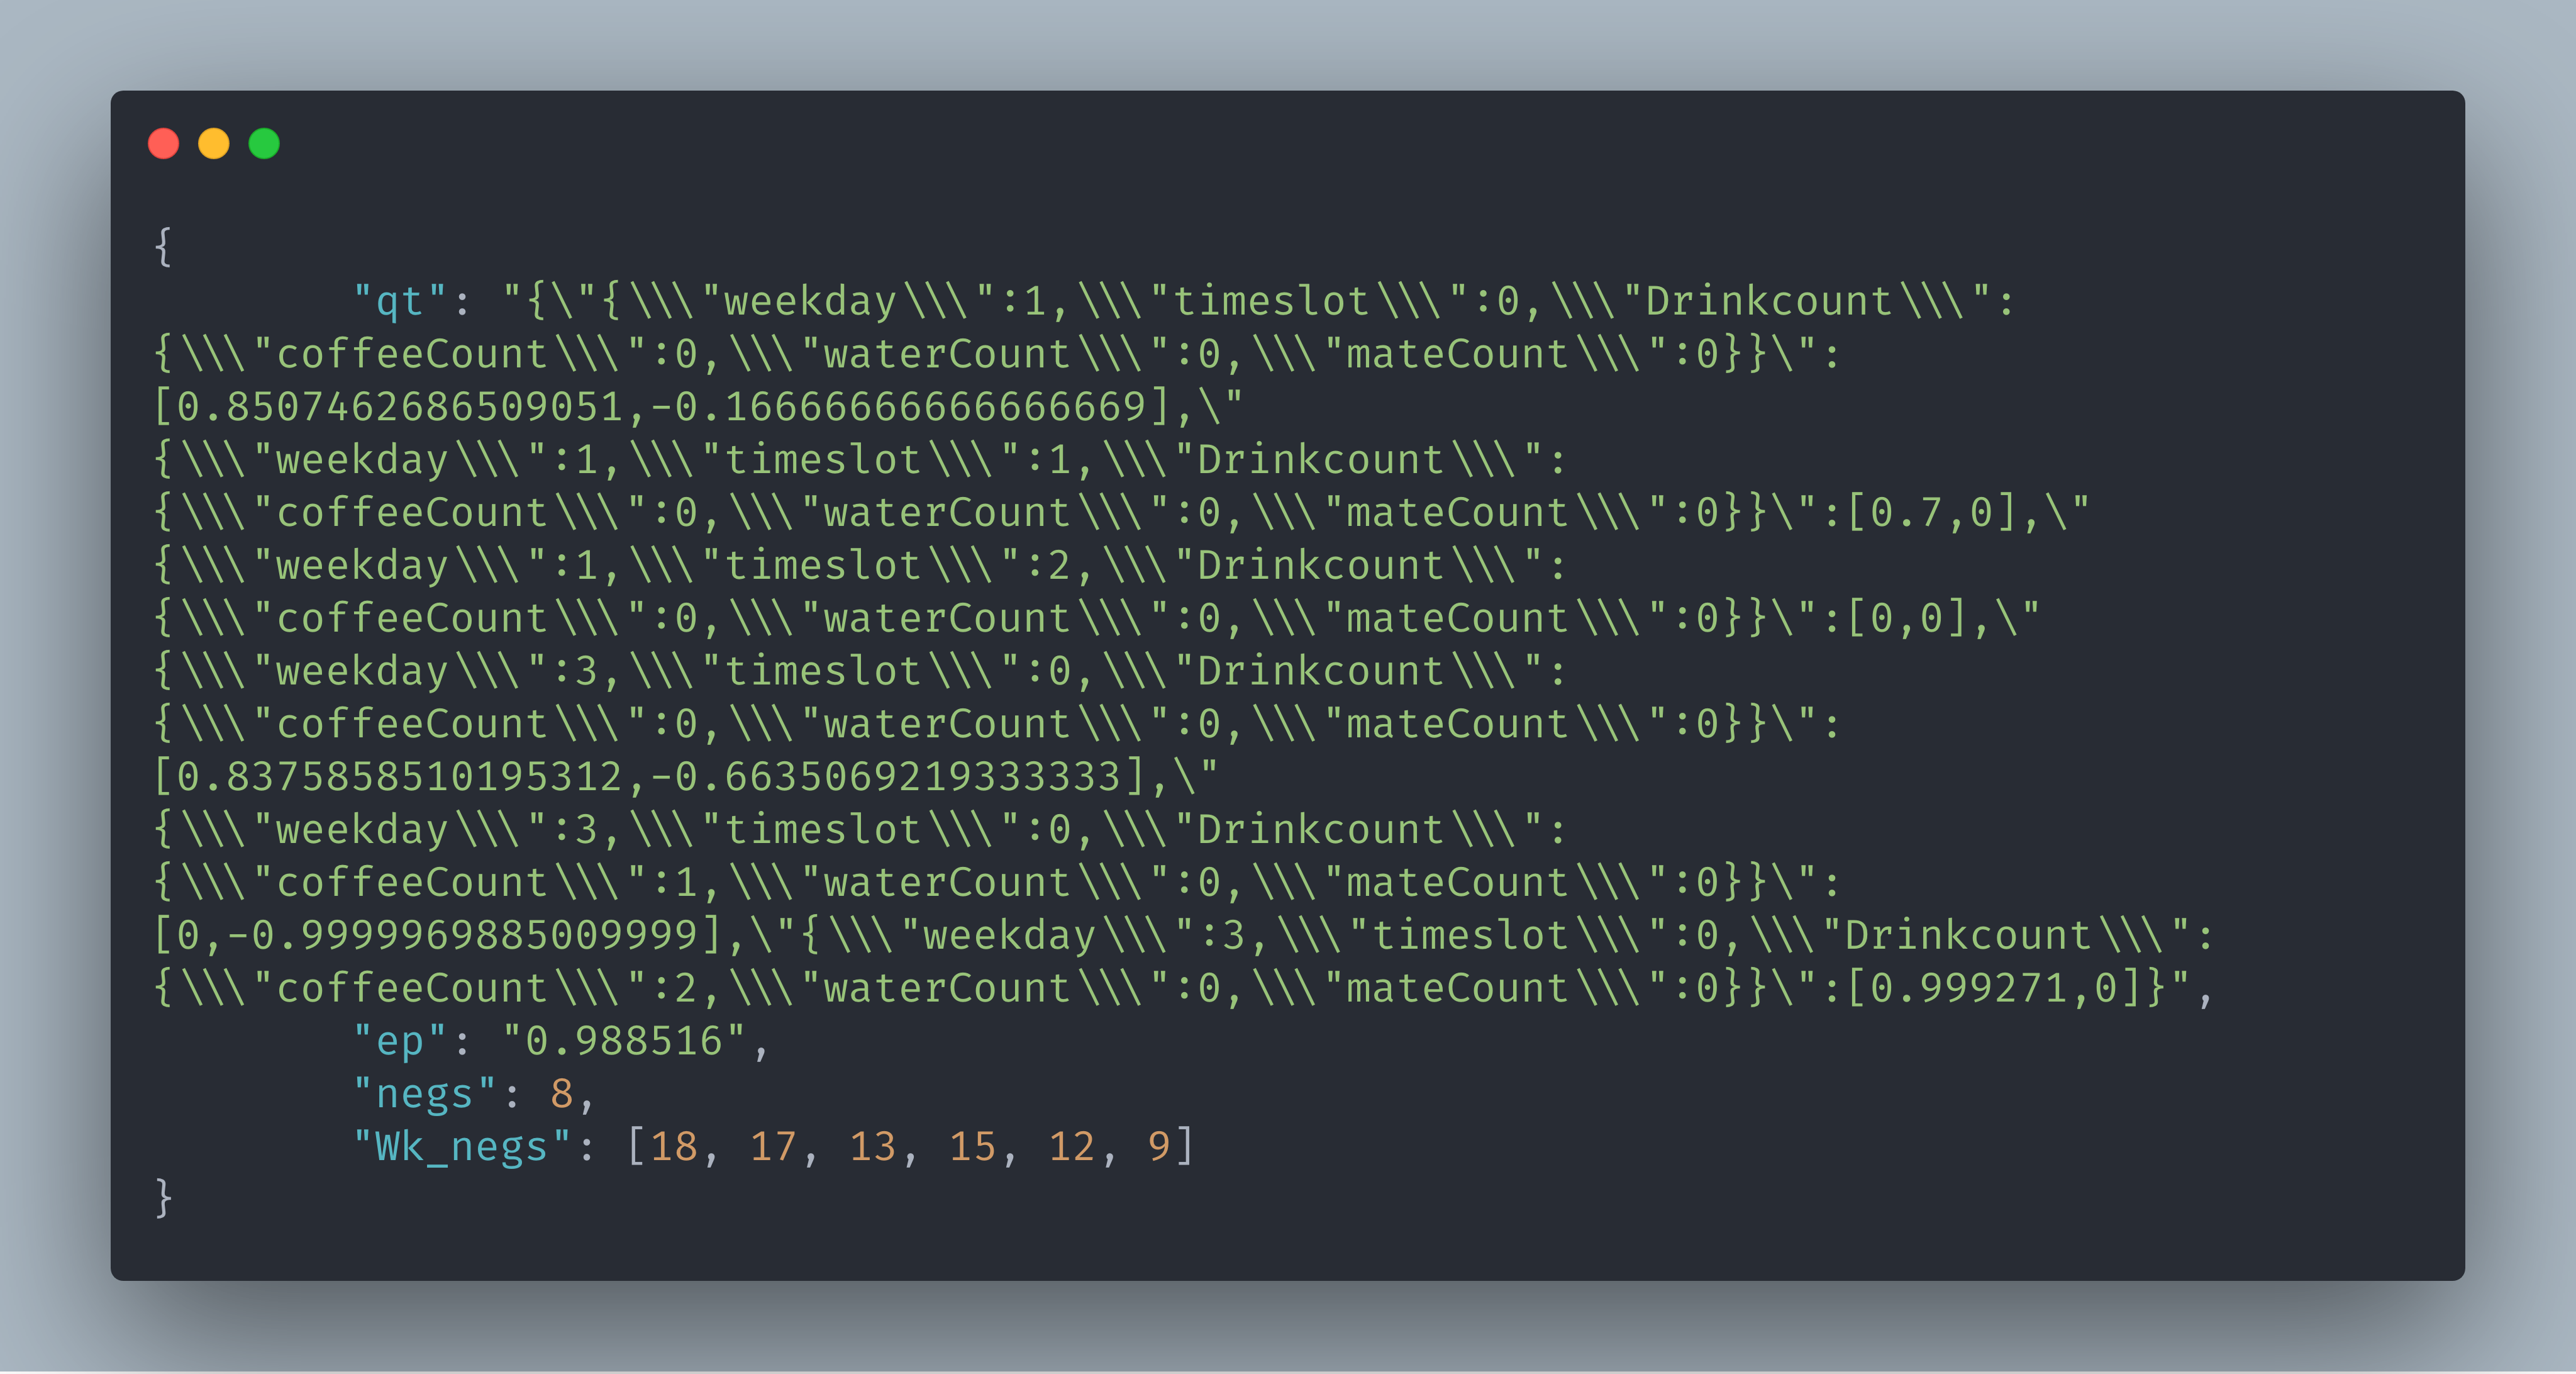
\includegraphics[width=.9\columnwidth]{./Abbildungen/Kapitel_03/usr_json.png}
	\caption{
		0x6ecbe1db9ef729cbe972c83fb886247691fb6beb-ql.json\\
		Der Name des JSON-Files setzt sich aus der Ethereum-Adresse des Users und der Abkürzung "ql", welches für Q-Learning steht, zusammenhängen.
	}
	\label{img:abb2}
\end{figure}

Der Vorteil liegt in der Möglichkeit den Learner jederzeit upzudaten ohne die gelernten Daten zu verlieren. Denn wird der Learner gestartet, holt sich dieser zuerst die Files vom Server, liest die Daten aus und initialisiert schon im Vorab die Q-Tabelle und das Epsilon eines jeden Users. \\
Sollte der Learner aus unbestimmten Gründen abstürzen, ist durch den eben beschriebenen Algorithmus die Erhaltung des Lernfortschrittes trotzdem sichergestellt.\\\\
Als letztes Modul wurde ein kleiner Node-Server entwickelt, dessen Aufgaben darin bestand die Smart-Contracts zu testen und als primitiver Ersatz für die App zu fungieren. Hierbei erzeugte er in einem festgelegten Intervall (7sek) Events mit einem zufällig generierten Daten (User \& Getränk) auf der Blockchain, um letztendlich die Event-Erkennung (“Watcher”) des “Learners” zu testen. Dabei wurde sowohl für den \quotes{Beverage-List Contract} als auch für den \quotes{CoffeeCoin-Contract} eine entsprechende Implementierung angefertigt.
\\In diesen Fällen wurde das Q-Learning-Submodul des Learners gar nicht erst gestartet, da lediglich die Funktionsweise des Watchers getestet werden sollte.\\
Besonders hier zeigte sich die Nützlichkeit des Fileservers, da gerade in der Entwicklungsphase die Smart-Contracts noch häufigen Änderungen unterlagen und dahingehend sehr oft neu deployed werden mussten, was ohne den Fileserver dazu geführt hätte die Smart Contract Daten bei jeder Iteration neu im Sourcecode zu hinterlegen.\\
Nach einer längeren Testphase, in der eine einwandfreie Kommunikation mit den beiden Smart Contracts attestiert werden konnte, wurde mit der eigentlichen Entwicklung der App begonnen, für jene auch Teile der Node-Server Implementierung übernommen werden konnten.\\
Schwierigkeiten traten dabei erst in der Testphase auf, in der festgestellt wurde, dass zu wenig Events vom Learner detektiert werden. Die Ursache dafür lag an der sehr alten Android Version des Tablets, die ist nicht ermöglichte eine direkte Verbindung zum Uni-Netzwerk herzustellen. Dies gelang nur mit einem Workaround, bei dem sich das Tablet mit einem öffentlichen Wlan-Netzwerk verband und sich daraufhin über eine VPN-Verbindung in das Uni-Netzwerk einwählen konnte. \\
Das führte jedoch dazu, dass die Verbindung zum Wlan-Netzwerk in unregelmäßigen Abständen abbrach und dadurch auch zur Blockchain. Da so ein unvorhergesehenes Verhalten wurde in der ersten Implementierung der App nicht vorgesehen war, musste dies in einem Update der App berücksichtigt werden (vgl. Kap. \ref{sec:app}), sodass keine Daten verloren gingen, sollte die Verbindung abbrechen. \\
Schlussendlich waren es sechs dedizierte Software Anwendungen, welche jeweils in eigenen Git-Repositories gehostet werden.
Dazu zählten:
\begin{itemize}
	\item Learner
	\item Tablet-App
	\item Go Fileserver
	\item Smart Contracts: Beverage-List, CoffeeCoin
	\item Web3 Node-Server
	\item Dockerimage für die Blockchain
\end{itemize}
Das Dockerimage fand in der Hinsicht keine größere Erwähnung, da es nur zu Test- und Weiterbildungszwecken entwickelt wurde und auch keine Verwendung in der finalen Architektur fand.


\section{Blockchain}
\label{sec:bchain}

Das folgende Kapitel erläutert im Detail den Setup der privaten Blockchain, sowie die beiden Smart Contracts welche ebenso ein Teil der Systemarchitektur darstellen.\\

\subsection{Genesis Block}
\label{subsec:genesis}
Der große Vorteil einer privaten (Ethereum) Blockchain gegenüber einer öffentlichen, ist die Möglichkeit die Blockchain nach den eigenen Vorstellungen und Anwendungszwecken zu konfigurieren. So können, wie auch bei einer öffentlichen Blockchain, Smart Contracts erstellt und Transaktionenen durchgeführt werden, allerdings ohne dabei wirkliches Ether zu besitzen. Denn eine Besonderheit eines sogenannten \quotes{Testnet's} ist das Erzeugen von \quotes{privatem} Ether, welcher Accounts zugeordnet und somit Transaktionenen durchgeführt werden können.\\
Die Konfiguration dessen erfolgt durch ein sog. \quotes{genesis.json file} (\ref{img:gen}). Diese Datei ist die Grundlage für den \textit{Genesis Block} der zu erstellenden Blockchain, welcher der erste Block in der Kette ist und somit auch keinen Vorgänger besitzt.\\\\
Das in \ref{img:gen} abgebildete JSON Objekt zeigt die in der Systemarchitektur verwendete Datei einen solchen \textit{Genesis Block} zu erzeugen. Nicht alle \quotes{properties} bedingen einer Erklärung, die essentiellen werden allerdings kurz erläutert: 

\begin{figure}[th!]
	\centering
	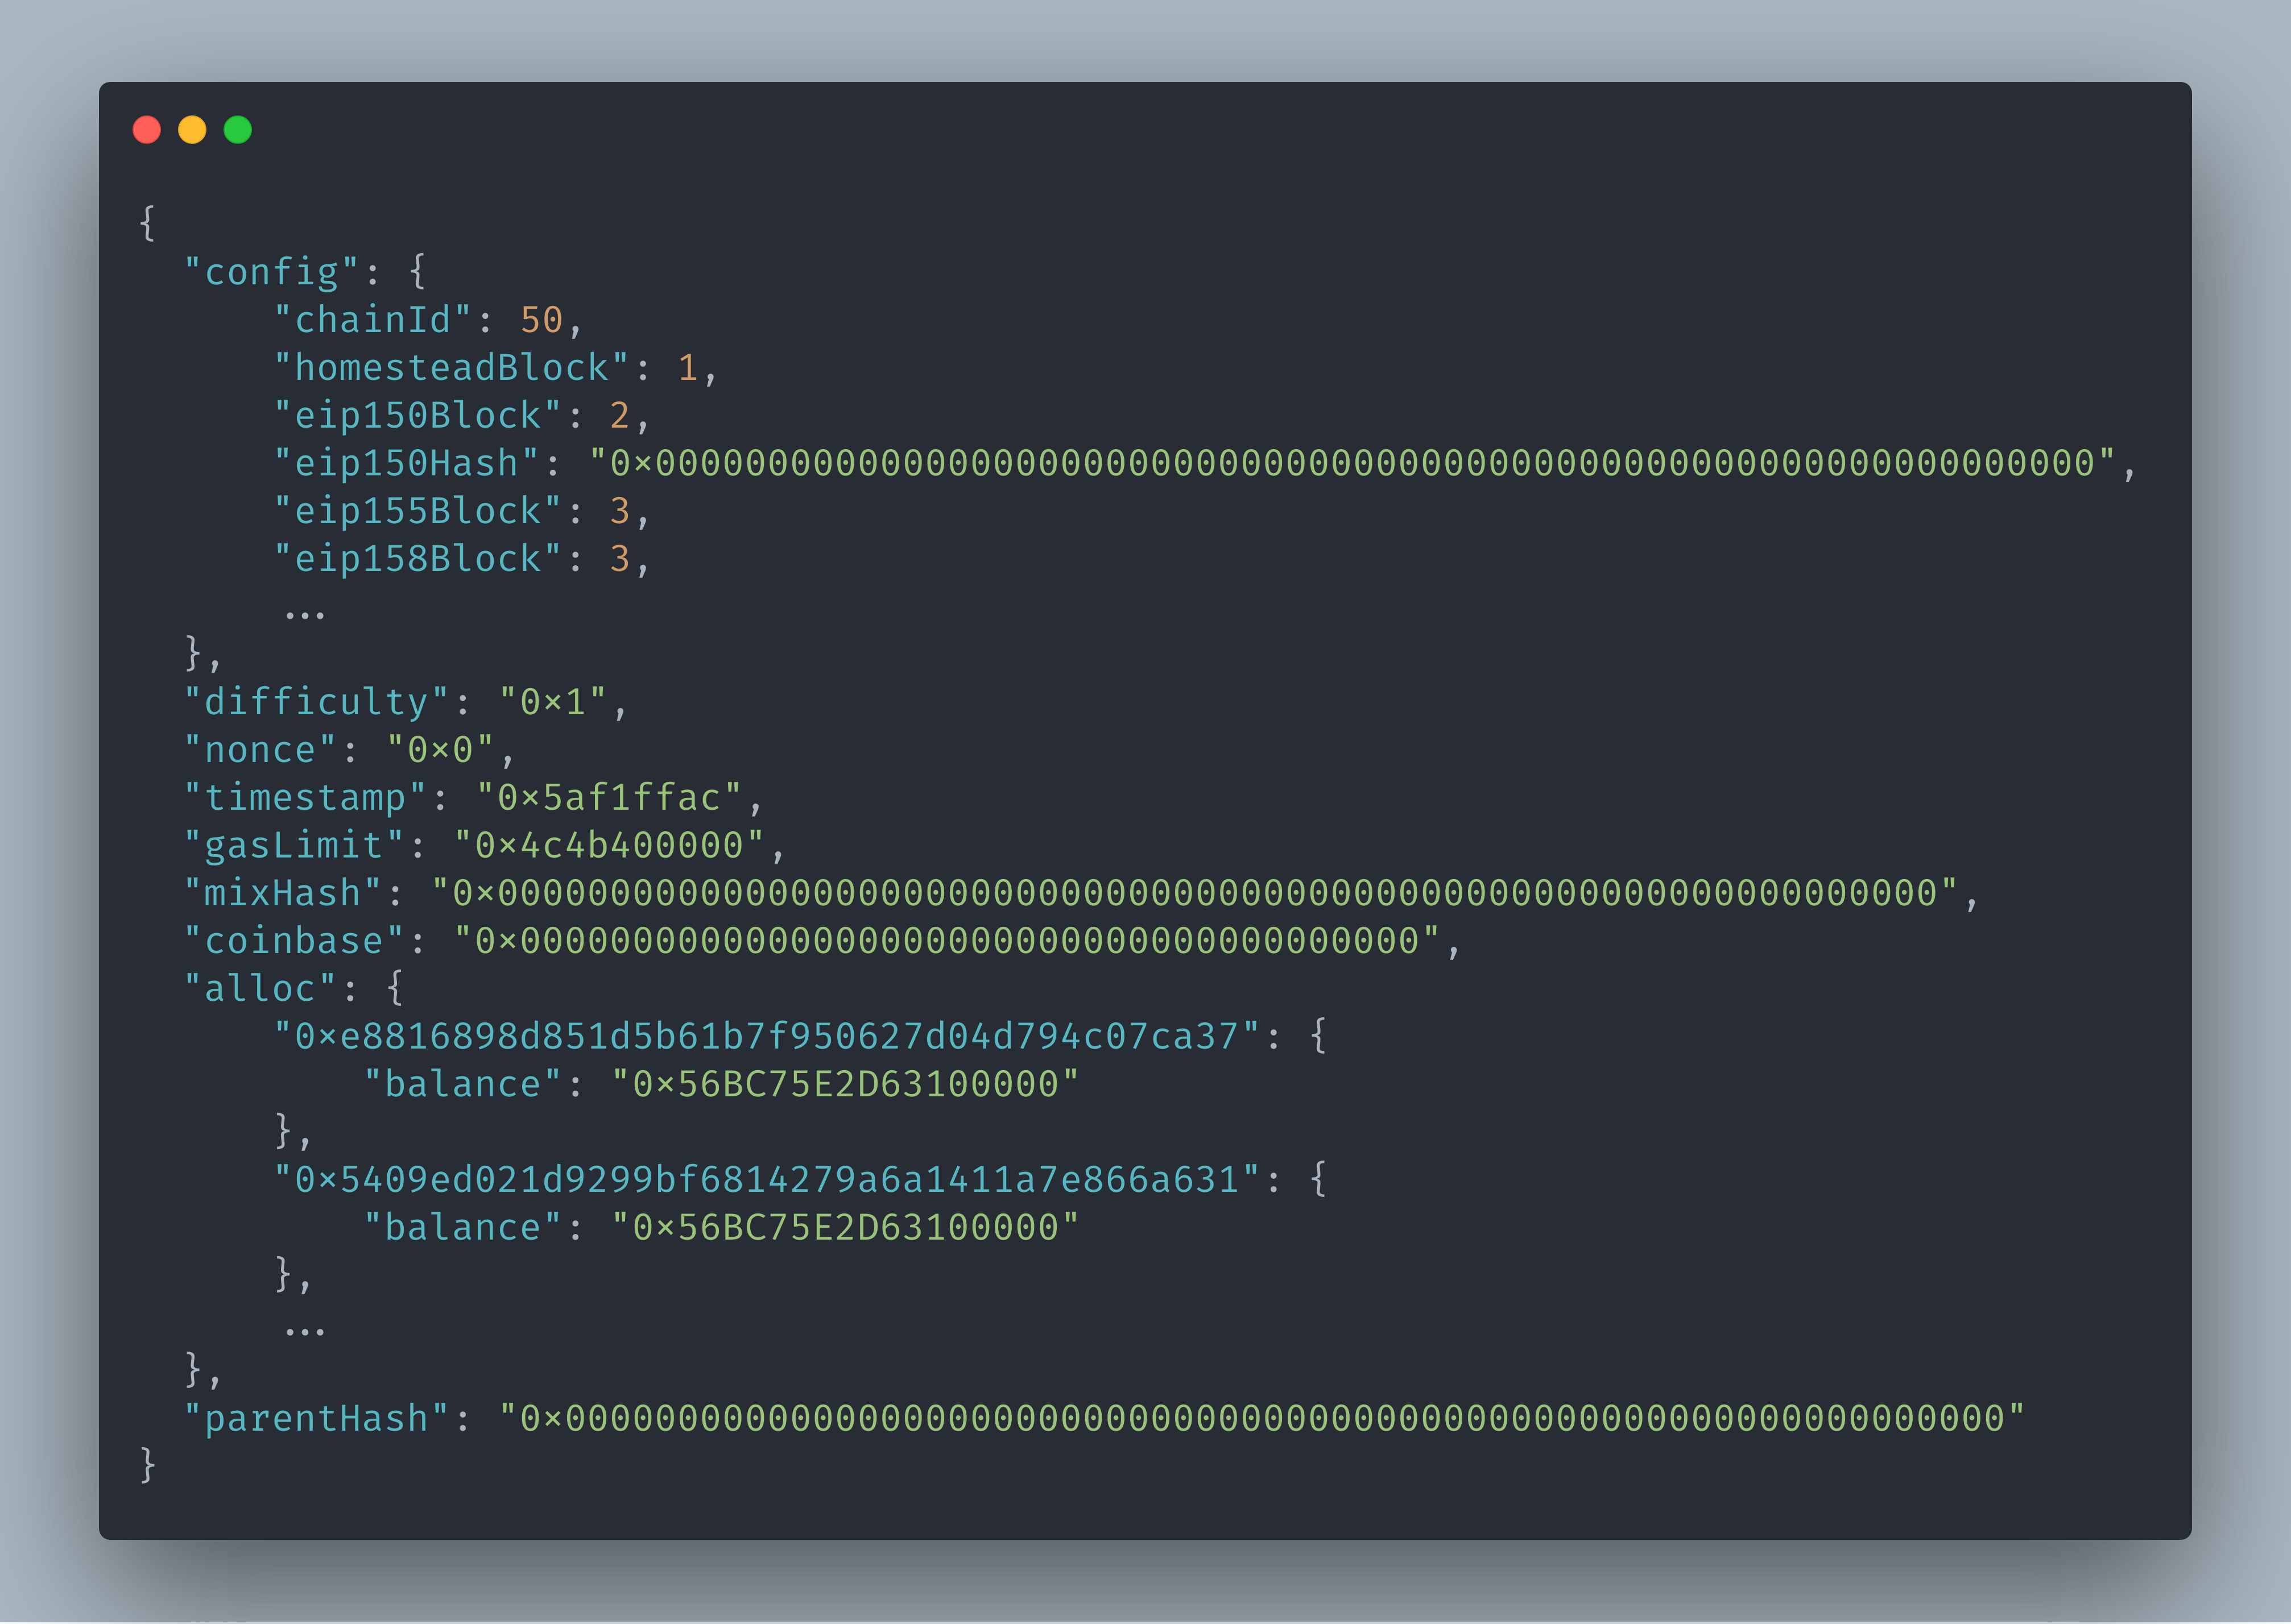
\includegraphics[width=.9\columnwidth]{./Abbildungen/Kapitel_03/genesis.json.png}
	\caption{
		genesis.json\\
		JSON-File welches zur Erstellung des Genesis Blocks verwendet wurde.
	}
	\label{img:gen}
\end{figure}

\begin{itemize}
	\item[-] chainId: ist eine einzigartige Id für die private Blockchain
	      	      	      	      
	\item[-] eip150Block/eip155Block/eip158Block: eip steht für \quotes{Ethereum Improvement Proposal}. Diese drei Community getriebenen \quotes{Proposals} beschreiben sog. \quotes{hard forks}, welche dafür sorgen sollten Fehler im Protokoll zu beheben. 
	      	      	      	      
	\item[-] homesteadBlock: Homestead ist die zweite \quotes{major version} von Ethereum, welche einige Änderungen an dem Protokoll vornahm
	      	      	      	      	
	\item[-] difficulty: beschreibt die Schwierigkeitsstufe für einen Miner einen validen Block zu finden. Das heißt je höher der Wert desto mehr Berechnungen müssen statisch durchgeführt werden und desto mehr Zeit wird benötigt, um eine Transaktion zu bestätigen. Im Falle eines Testnets ist es deshalb ratsam einen sehr niedrigen Wert zu wählen
	      	      	      	      	
	\item[-] gasLimit: beschreibt das Limit für eine Transaktion wie viel an Gas verbraucht werden darf. 
	      	      	      	      
	\item[-] alloc: hier können Accounts schon im Voraus mit \quotes{fake ether} befüllt werden.
	\item[-] nonce: ist ein Zähler für die Anzahl der durchgeführten Transaktionen einer Adresse
\end{itemize}

Sobald die genesis.json Datei fertiggestellt ist, kann die Blockchain mit folgendem Befehl erstellt werden:\\\\
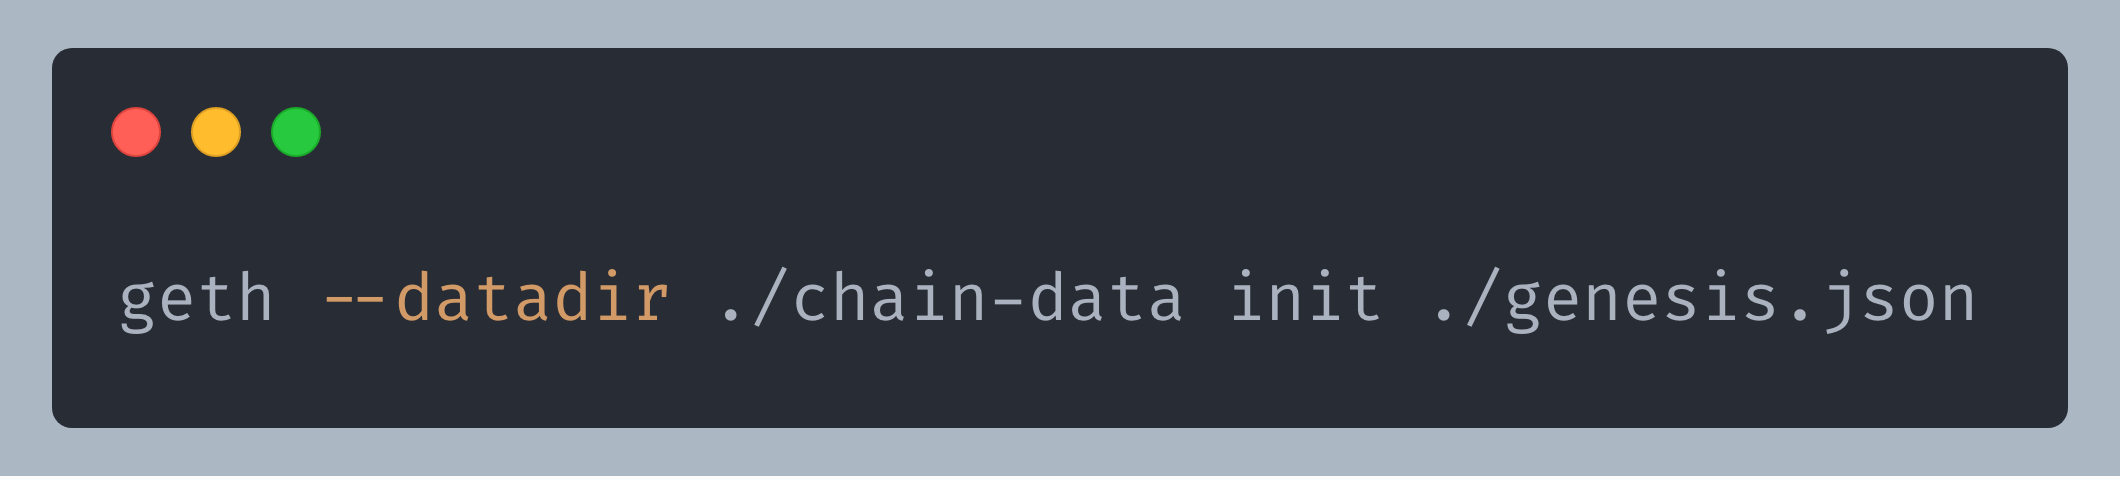
\includegraphics[width=.9\columnwidth]{./Abbildungen/Kapitel_03/geth-init.png}

Das Flag \textit{-{}-datadir} ist mit dem aus Abbildung \ref{img:geth} identisch. Das bedeutet das Verzeichnis welches hier im Befehl angegeben ist, muss beim Kommandozeilenbefehl in Abbildung \ref{img:geth} exakt gleich sein. Andernfalls ist es nicht möglich die Blockchain zu starten.\\\\
Nachdem der Setup der privaten Blockchain abgeschlossen ist, kann mit der Entwicklung eines Smart Contracts begonnen werden. \\
Die nächsten beiden Unterkapitel befassen sich mit den Smart Contracts, welche im Zuge dieser Arbeit entwickelt wurden.

\subsection{CoffeeCoin}
\label{subsec:cc}
Der Smart Contract \quotes{CoffeeCoin} stellt einen sogenannten ERC-20 Token mit gewissen Abwandlungen dar. Dabei ist ein Token im Grunde eine zusätzliche Währung zur eigentlichen Währung von Ethereum dem Ether. Das bedeutet Smart Contracts können somit eine eigenständige Währung abbilden. Für solche Smart Contracts gibt es mittlerweile einige Standardisierungen, die Vorschreiben welche Methoden und Datenstruktur ein Smart Contract zu implementieren hat. Der am weit verbreitetste Standard ist der ERC-20, bei welchem es folgende Funktionen und Events zu implementieren gilt:

\begin{figure}[th!]
	\centering
	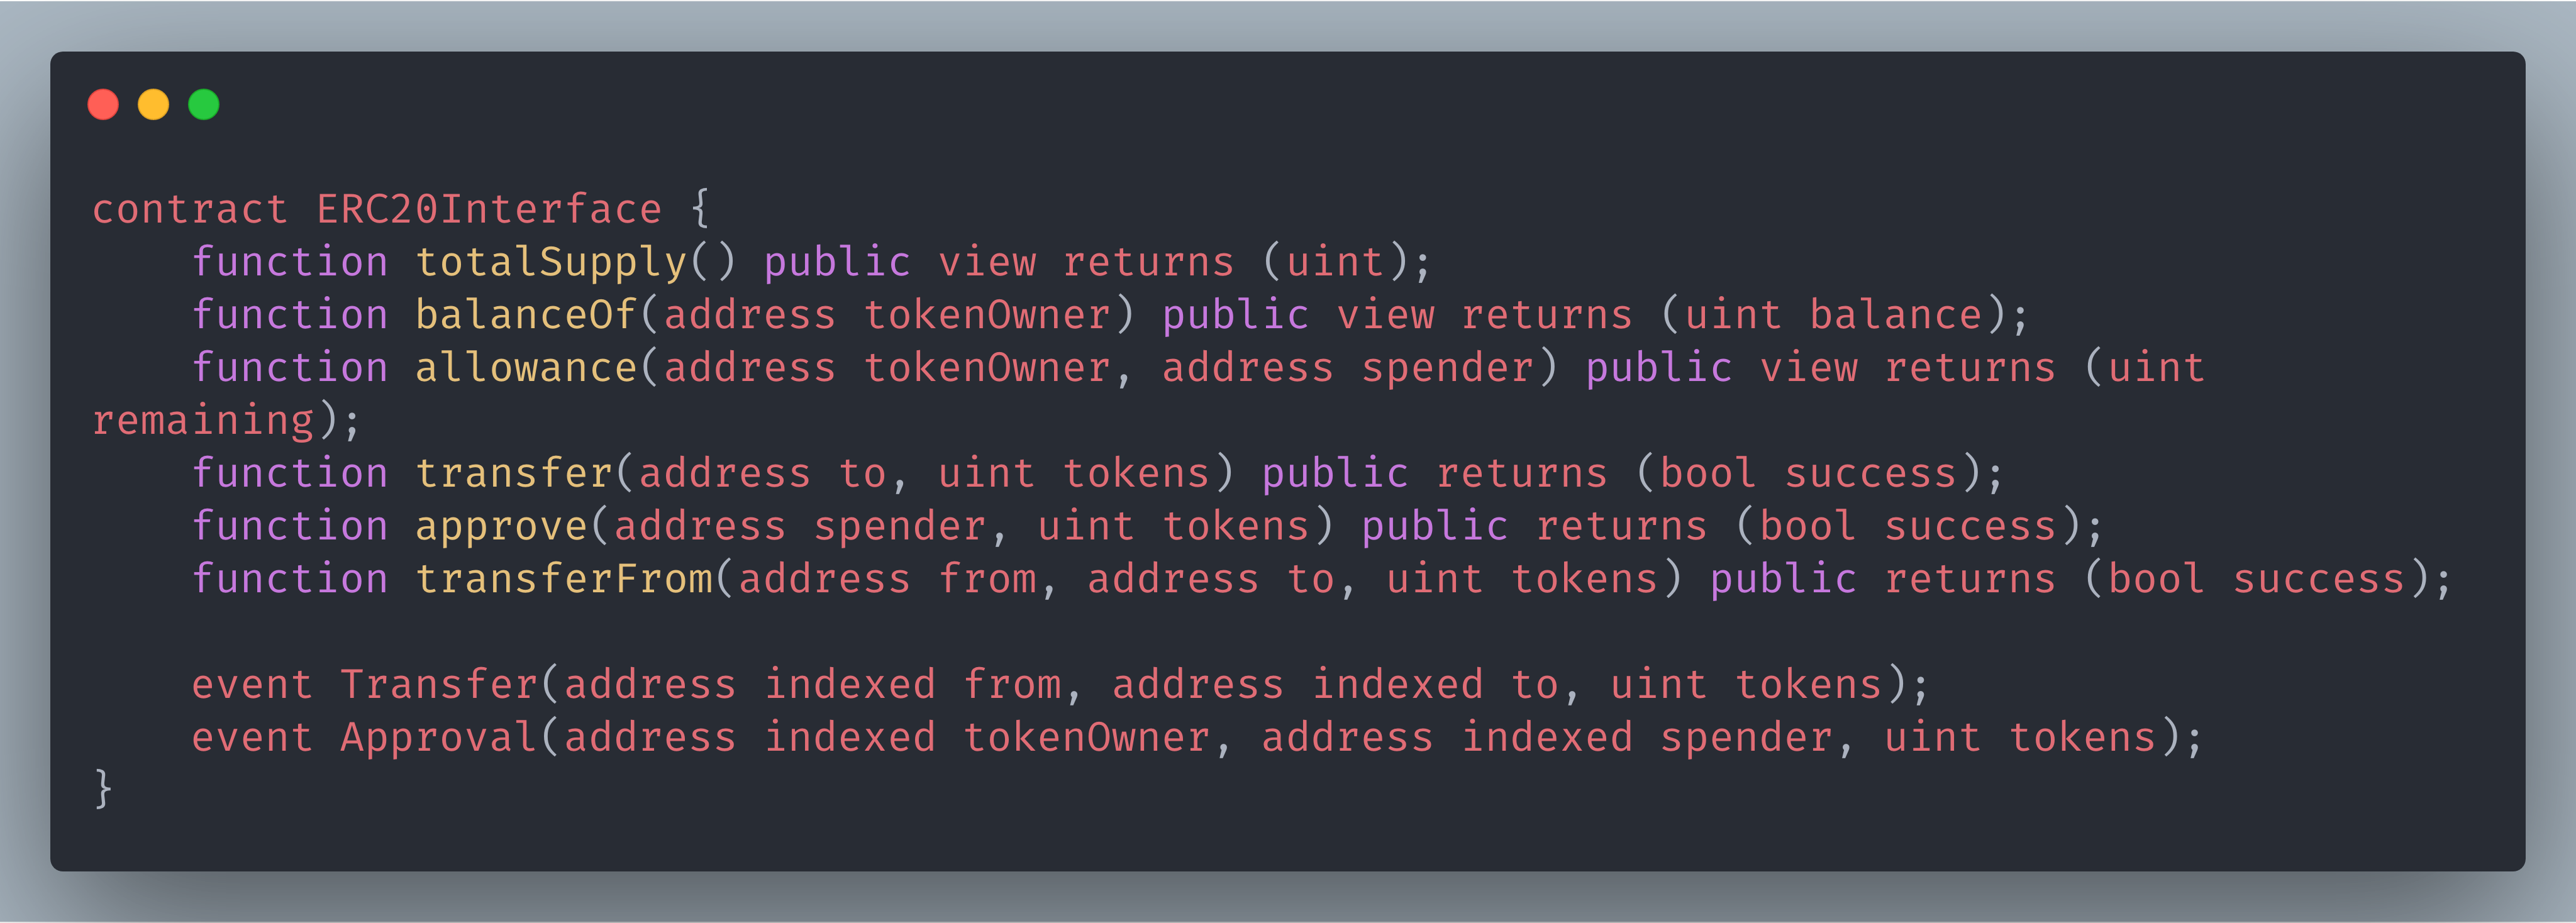
\includegraphics[width=.9\columnwidth]{./Abbildungen/Kapitel_03/erc20.png}
	\caption{ERC-20 Interface}
	\label{img:gen}
\end{figure}

\begin{itemize}
	\item totalSupply: Gesamtanzahl der existierenden Tokens
	\item balanceOf: Anzahl der Tokens eines bestimmten Users
	\item allowance: besagt wie viele Tokens eines bestimmten Users durch einen bestimmten \quotes{spender} abgehoben werden dürfen
	\item transfer: transferiert die Inputanzahl an Tokens des \quotes{senders} (Adresse welche diese Funktion aufgerufen hat) an die angegebene Adresse
	\item approve: Erlaubniserteilung an den \quotes{spender} die in \textit{allowance} festgelegte Anzahl an Tokens abzubuchen
	\item transferFrom: transferiert die angegebene Anzahl von Tokens von der \quotes{from Adresse} zur \quotes{to Adresse}
	\item event Transfer: wird von den beiden \textit{transfer} Funktionen ausgelöst
	\item event Approval: wird von der \textit{approve} Funktion ausgelöst
\end{itemize}

Der eben erläuterte Token Standard wurde im Falle des CoffeeCoin Smart Contracts um zusäztliche Funktionen und Datenstrukturen erweitert. Diese Erweiterungen stellen eine gesonderte Abstraktionsebene nach außen hin da, um die Kommunikation seitens der Tablet-App zu erleichtern und einfacher zu gestalten.\\
So werden schon beim Deployment die einzelnen Preise der Getränke und die Adresse, zu jener die Tokens beim Bezahlen eines Getränks überwiesen werden, gesetzt.\\
Dies ermöglicht die Implementierung folgender Funktionen: 

\begin{figure}[th!]
	\centering
	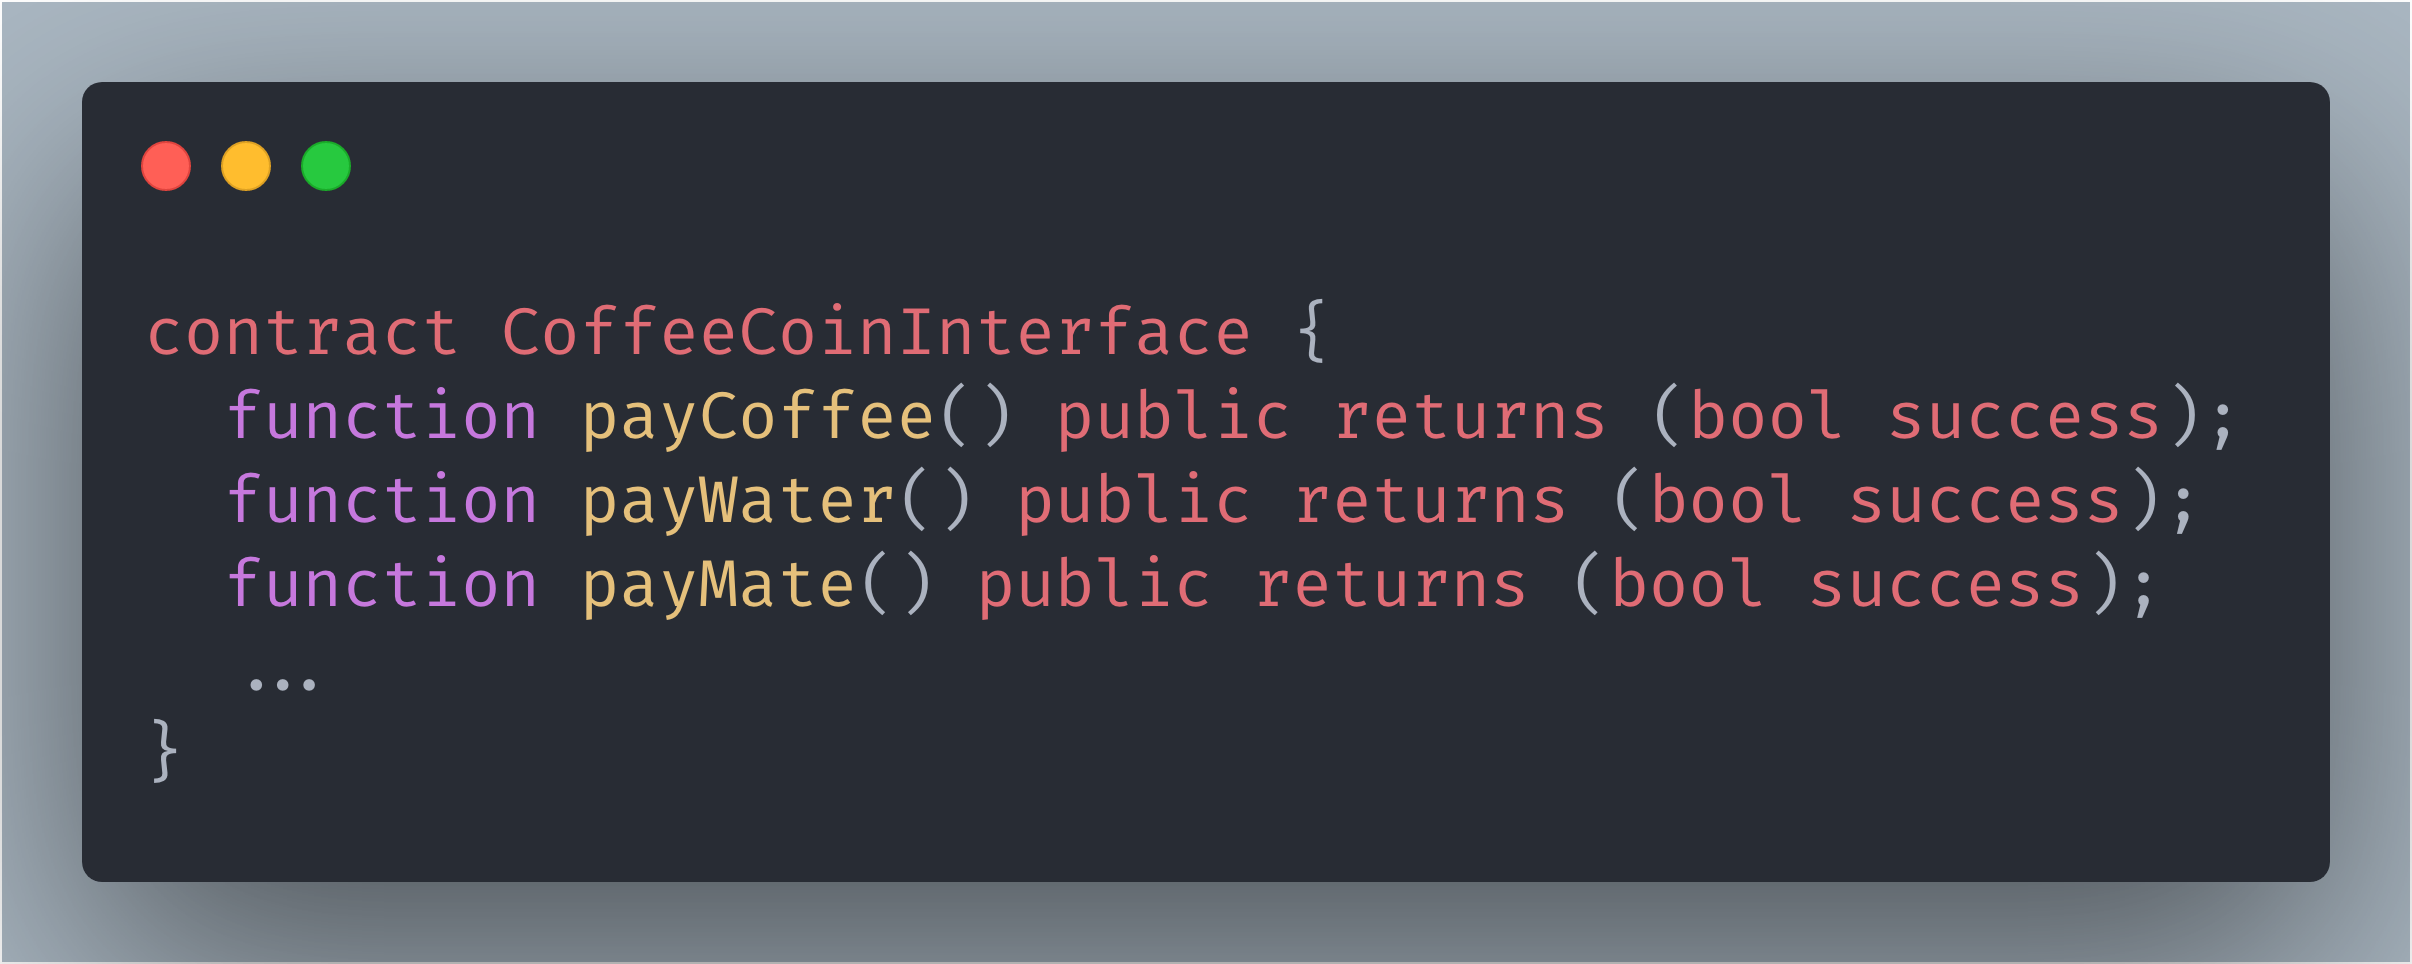
\includegraphics[width=.9\columnwidth]{./Abbildungen/Kapitel_03/CCInterface.png}
	\caption{CoffeeCoin Interface Auszug}
	\label{img:cci}
\end{figure}

Diese Funktionen bieten eine Abstraktionsebene zur ERC-20 Funktion \textit{transferFrom}. Da bereits beim Deployment die Parameter für die Getränke und die Zieladresse gesetzt werden, benötigen diese Funktionen keine weiteren Daten von der Seiten der User (Tablet-App). Somit kann nach Auswahl des Getränks die entsprechende Funktion aufgerufen werden, ohne sich dabei mit den Details der Transaktion beschäftigen zu müssen.\\\\
Desweiteren wird einem User, beim ersten Aufruf einer jener Funktionen (erste ausgelöste Transaktion des Users), eine festgelegte Anzahl an Tokens als \quotes{Startguthaben} überwiesen, sodass dieser stets über genügend Token verfügt und jederzeit Transaktionen durchführen kann.\\
Im Kontext der Problemstellung liegt die Zweckmäßigkeit des Smart Contracts grundsätzlich in der Bezahlung der Getränke in Form des Tokens. Dabei soll vor allem die Möglichkeit einer solchen Bezahlmethode aufgezeigt werden, weswegen die Transaktionen lediglich auf exemplarischer Ebene durchgeführt werden. Das bedeutet, den Usern wird, wie gerade beschrieben, eine nahezu unendliche Menge an Tokens zugewiesen ohne eine Gegenleistung zu fordern.\\\\
Der Sourcecode ist im Anhang unter REF SO UND SO zu finden.


\subsection{Beverage-List}
\label{subsec:bl}

Im Gegensatz zur CoffeeCoin basiert der Beveragelist Contract auf keinem festgelegten Standard, sondern ist in voller Gänze an die Problemstellung angepasst.\\
Dessen Zweck besteht im Grunde darin eine Getränkeliste abzubilden, in welcher jede Getränktransaktion eines Users vorzufinden ist. Dabei wird pro Transaktion nicht nur das Getränk, sondern auch das aktuelle Datum inklusive Uhrzeit und der aktuelle Wochentag, gespeichert. Diese Daten sollen es dem Learner schlussendlich ermöglichen das Kaffeetrinkverhalten des Users zu erlernen. \\
Damit der Learner ohne großen Aufwand auf diese Informationen zugreifen kann, löst der Smart Contract, mit den eben genannten Daten beinhaltend, ein Event aus, sobald seine Methode \quotes{setDrinkData} aufgerufen wird. Diese Funktion 
hinterlegt die übergebenen Daten (Eth-Adress, Zeit, Wochentag, Getränk) in festgelegten Datenstruktur und löst zugleich das Event für den Learner aus.\\\\

Dieser Smart Contract umfasst noch weitere Funktionen, welche aber vor allem zu Testzwecken implementiert wurden und in der finalen Systemarchitektur keine Verwendung finden. 


\section{Learner}
\label{sec:ql}
Als nächstes wird der sogenannte \quotes{Learner} detailiert betrachtet. Dabei wird zuerst die Problemstellung hinsichtlich des Reinforcement-Learnings modelliert und im Anschluss der verwendete Algorithmus (Q-Learning) allgemein und im Kontext der Problemstellung erläutert. \\

\subsection{Modellierung}
\label{subsec:modulation}
Die Modellierung eines Lernproblems im Hinblick auf einen Reinforcement-Algorithmus erfolgt in der Regel stets nach der selben Systematik. \\
Dabei werden zuerst der Zustandsraum, also alle möglichen Zustände, alle Aktionen des \quotes{Agenten} und der Reward für ausgeführte Aktionen eruiert.
Hier in diesem Fall ist der Agent der Learner, welcher das Kaffeetrinkverhalten der User zu erlernen versucht.\\\\
Die Modellierung sieht wie folgt aus: 
\paragraph{Zustandsraum}
\begin{itemize}
	\item Wochentag: Montag, Dienstag, Mittwoch, Donnerstag, Freitag
	\item Timeslot:
	      \begin{itemize}
	      	\item 7-9 Uhr (T0)
	      	\item 10-12 Uhr (T1)
	      	\item 13-15 Uhr (T2)
	      	\item 16-18 Uhr (T3)
	      	\item 19-6 Uhr (T4)
	      \end{itemize} 
	\item Kafee-Anzahl: n $*$ Kaffee (n=Anzahl pro Tag)
\end{itemize}

\paragraph{Aktionen}
\begin{itemize}
	\item Kaffee
	\item Nothing
\end{itemize}

\paragraph{Reward}
\begin{itemize}
	\item +1 bei richtiger Prediction
	\item \textminus 1 bei falscher Prediction
\end{itemize}
\ \\
Daraus lässt sich folgender examplarischer Zustand konstruieren: 
\begingroup
\makeatletter
\@totalleftmargin=0.5cm
\begin{Verbatim}
	< Wochentag: Montag; Timeslot: 2; Kaffee-Anzahl: 3 >
\end{Verbatim}
\endgroup
Das bedeutet konkret: an einem Montag wurden einschließlich des 2. Timeslots (13-15 Uhr) 3 Kaffee getrunken. Dieser Status gibt jedoch keinen Aufschluss darüber, welcher sein Vorgänger war und welcher sein Nachfolger sein wird. So können einerseits alle Kaffee's nur in Timeslot 2 getrunken worden sein oder in jedem Timeslot (0,1,2) jeweils einen. Andererseits besteht auch die Möglichkeit, dass im Timeslot 2 nochmals ein Kaffee konsumiert wird oder eben erst in einem nachfolgendem Timeslot.\\
Dieses Lernproblem ist auch als \quotes{Multi-Armed Bandit Problem} bekannt und wird in Kap. \ref{subsec:y-ql} erläutert.
\\\\
Der erste Modellierungansatz sah anstatt der Kaffe-Anzahl eine Getränkeanzahl vor, bei der zum Kaffee auch die Quantität der getrunkenen \quotes{Clube Mate} und \quotes{Wasser} berücksichtigt werden sollten. Der Grund dafür liegt in dem erheblichen Einfluss des Konsums weiterer Getränke auf das Kaffeetrinkverhalten, wodurch mit solch einer granularen Modellierung genauere Predictions zu erwarten sind. Jedoch steigt somit auch die Anzahl der zu durchlaufenden Zustände und einhergehend die zu erlernenden optimalen Aktionen für die Zustandsübergänge. Letztlich resultiert dies in der längeren Trainingsphase des Algorithmus, was aber aufgrund des zeitlich begrenzten Rahmen dieser Arbeit nicht durchführbar war und deshalb der Ansatz mit lediglich der Kaffee-Anzahl gewählt wurde.\\

TO-DO: feature selection to add
user versteht zu jeder warum algorithmus so handelt

\subsection{Q-Learning}
\label{subsec:y-ql}
Der Q-Learning Algorithmus fällt unter die Methodik des TD-Learnings (vgl. \ref{subsec:rl}). Der Algorithmus wartet aus diesem Grund nicht bis zur Terminierung einer Episode, um die Wertfunktion zu schätzen, sondern berechnet diese im nächsten Zeitschritt. Im Gegensatz zu anderen TD-Learning Algorithmen bemisst die Wertfunktion des Q-Learning nicht den aktuellen Zustand, hingegen  beurteilt es die Aktion in diesem Zustand. Hierbei wird von der Aktion-Wert Funktion Q gesprochen. \\\\
Die Berechnung von Q erfolgt nach folgender Formel (\ref{eqn:qval}):
\begin{equation}
	\label{eqn:qval}
	$Q(s_t,a_t)\;\leftarrow\;Q(s_t,a_t) + \alpha [ r_{t+1} + \gamma \max_a
	Q(s_{t+1},a) - Q(s_t,a_t) ]$
\end{equation}
\begin{itemize}
	\item Q(s\textsubscript{t},a\textsubscript{t}): beschreibt den aktuellen Q Wert bzw. Q-Value der Aktion a welche zum Zeitpunkt t im Zustand s ausgeführt wurde
	\item \textalpha: wird als Lernrate bezeichnet und gibt an in welchem Maße der alte Q-Value durch den Neuen überschrieben wird
	\item r\textsubscript{t+1}: ist der Reward zum Zeitpunkt t+1, nachdem im Zustand s die Aktion a ausgeführt worden ist
	\item \textgamma: ist der Diskontierungsfaktor und wird als Gewichtung für zukünftige Rewards verstanden 
	\item max\textsubscript{t}Q(s\textsubscript{t+1},a\textsubscript{t}): ist das Maximum an Reward, der durch die Ausführung der Aktion a' im neuen Zustand s' erfolgt
\end{itemize}

Abgespeichert werden diese Q-Values in der sogenannten Q-Tabelle (vgl. \ref{table:qtable}), hierbei gibt es ein 1:1 Mapping von jeweils einem Zustand auf jeweils eine Aktion. 

\begin{table}[h!]
	\begin{center}
		\caption{Exmplarische Q-Tabelle}
		\begin{tabular}{| l | l | l | l |}
			\hline
			    & a1  & a2   & a3  \\ \hline
			s1  & 0.1 & -0.2 & 1.2 \\ \hline
			s2  & 0.4 & -0.5 & 0.8 \\ \hline
			s3  & 1.1 & -0.3 & 0.7 \\ \hline
			... & ... & ...  & ... \\ \hline
		\end{tabular}
		\label{table:qtable}
	\end{center}
\end{table}

Die Anwendung und der Ablauf wird anhand des Pseudocodes in Algorithmus \ref{ql-psc} abgebildet.

\begin{algorithm}
	\caption{Q-learning algorithm}\label{euclid}
	\label{ql-psc}
	\begin{algorithmic}[1]
		\State Initialize Q(s,a), for all s \textepsilon S,a \textepsilon A(s) and Q(terminal-state,·) = 0
		\Repeat (for each episode):
		\State Initialize s
		\Repeat (for each episode):
		\State Choose A from s using policy derived from Q (e.g., greedy)
		\State Take action A, observe R, s'
		\State $Q(s_t,a_t)\;\leftarrow\;Q(s_t,a_t) + \alpha [ r_{t+1} + \gamma \max_a
		Q(s_{t+1},a) - Q(s_t,a_t) ]$
		\State s $\leftarrow $ s' 
		\Until s is terminal
	\end{algorithmic}
\end{algorithm}

Zum Start wird der Q-Table initialisiert, indes jedes Feld eines Zustand-Aktions-Paars auf '0' gesetzt wird. Im Anschluss wird ein Durchlauf mit einer bestimmten Anzahl an Episoden gestartet. Hierbei wird zunächst der aktuelle Zustand initialisiert bzw. beobachtet und daraufhin eine weitere Schleife betreten, welche solange durchlaufen wird bis der Zustand s terminiert. Als nächstes wird eine Aktion a anhand der aktuellen Strategie ausgewählt. Diese Aktion wird ausgeführt und der resultierende Reward, sowie der neue Zustand werden detektiert. Anhand dieser Beobachtung wird mit der Formel (vgl. \ref{qval:formula}) der neue Q-Value berechnet und die Q-Tabelle upgedatet. Zum Schluss wird der neue Zustand s' als der 
aktuelle Zustand s gesetzt und eine neue Iteration beginnt. \cite{Sutton, mlmitchel, MultiagentSystems} \\\\
Der gerade eben beschrieben Algorithmus findet sich in einer abgewandelten Form in der Implementierung des \quotes{Learners} wieder. So wird eine Aktion nicht immer nach dem greedy-Prinzip der Reward-Maximierung ausgewählt, sondern nach der Methodik des \textepsilon-greedy. Dabei beschreibt die Variable \textepsilon einen Wert zischen '0' und '1' und gibt dadurch das Verhältnis zwischen Exploration und Exploitation an - in der Regel ist der Wert von \textepsilon eher klein. So wird im Falle von \text{MaxQ} stets die Aktion a ausgeführt welche in Zustand s den größten Reward verspricht - auch als greedy Strategie bekannt. Bei \textepsilon-greedy jedoch, wird zu einem gewissen Anteil - definiert durch das \textepsilon - nicht immer die Aktion ausgewählt welche den größten Reward verspricht, sondern eine Aktion zufällig selektiert,  obgleich des erwarteten Rewards. Somit wird eine Erforschung des Zustandsraum durch den Lernagenten sichergestellt und eine Beschränkung auf lediglich bekannte Aktionen und Zustände vermieden. \\
Eine Besonderheit der Implementierung liegt in der Vakanz der Berücksichtigung von Folgezuständen in der Berechnung des Q-Values.
\begin{equation}
	\label{eqn:bandit}
		$Q(s_t,a_t)\;\leftarrow\;Q(s_t,a_t) + \alpha [ r_{t+1} - Q(s_t,a_t) ]$
\end{equation}

Aufgrund der In­de­pen­denz der Zustände untereinander, ist das Verfolgen einer Strategie und das Einbeziehen der Folgezustände in die Berechnung der Q-Werte nicht notwendig. Der Fokus wird dadurch nur auf den Zustand als solches gelegt und die Annäherung des \quotes{wahren} Q-Wertes indessen einzig anhand des Rewards r\textsubscript{t+1} durchgeführt. \\
Diese Form der Problemstellung wird auch als \textit{n-armiger Bandit} Problem bezeichnet. Dieses ist ein klassisches Problem des Reinforcement Learning, welches das Dilemma zwischen Exploration und Exploitation aufdeckt. Es beschreibt das Spielen an mehreren (n) Glücksspielautomaten, deren einzige Aktion die Betätigung des Hebels ist. Das Ziel das Spielers ist es seine Belohnung zu maximieren (Exploitation) und wird deswegen nach jeder Aktion vor die Entscheidung gestellt, ob der Wechsel zu einem anderen Automat einen größeren Gewinn für ihn bedeutet (Exploration) oder ob er den aktuellen beibehält. \\
Die Analogie zum Lernproblem besteht in der Abbildung des unmittelbaren Rewards auf die gewählte Aktion. Eine Aktion wird nie anhand von nachfolgenden Aktionen bewertet, sondern einzig anhand der Belohnung nach ihrer Ausführung. Außerdem handelt es sich in beiden Fällen um ein nichtdeterministisches Lernproblem, bei welchen die Ausführung einer Aktion in einem bestimmten Zustand stets einen Reward nach einer Wahrscheinlichkeitsverteilung nach sich zieht und somit eine hundertprozentige Vorhersage der zu erhaltenden Belohnung nicht möglich ist. \cite{Sutton}
	
\subsection{Lernprozess \& Ablauf}
\label{subsec:learning}

Aufgrund der Modellierung eines Zustandes ergeben sich zwei Arten bei denen eine Änderung dessen hervorgerufen wird: 
\begin{itemize}
	\item durch eine zeitliche Komponente, bei der sich entweder der Timeslot oder der Tag ändert
	\item durch den User indem er eine Transaktion auslöst
\end{itemize}

Das ist in der Hinsicht von großer Bedeutung, da für diese Übergänge ein Feedback für den Agenten notwendig ist, um jeweils die optimale Aktion dafür zu erlernen. \\
So wird das Feedback einerseits von Seiten des Users in Form einer bestätigten Transaktion generiert, was bedeutet Aktion \quotes{Kaffee} wurde ausgeführt. Oder andererseits als Folge einer fehlenden Rückmeldung des Nutzers, welche \quotes{Nothing} als optimale Aktion impliziert. \\
Das heißt erfolgt eine Zustandsänderung durch den User, so ist stets \quotes{Kaffee} die zu erlernende, beste Aktion. Wird eine Zustandsänderung durch einen Timeslotwechsel bewirkt, so ist das Feedback der Umgebung immerfort die Aktion \quotes{Nothing}. \\
Um dem Agenten bzw. dem Q-Learning Algorithmus stets das nötige Feedback zu geben und Zustandsübergänge herbeizuführen, werden im Learner die Komponenten \quotes{Watcher} und \quotes{Worker} verwendet. \\
Der \quotes{Watcher} ist dafür zuständig das Feedback des Users durch das Beveragelist-Event zu detektieren und die darin enthaltenen Daten dem Algorithmus zur Verfügung zu stellen. \\
Der \quotes{Worker} wird für die zeitliche Komponente verwendet, indem er am Ende jedes Timeslots aktiv wird, die Zustandsänderung durchführt und dem Agenten die Aktion \quotes{Nothing} als Feedback gibt. \\
Auf Basis dieser Feedbacks wird es dem Q-Learning Algorithmus ermöglicht die optimalen Aktionen zu erlernen. Hierbei wird die Prediction, also die aus Sicht des Agenten beste Aktion für den Zustandsübergang, anhand der Rückmeldung, sei es durch den Watcher oder Worker, evaluiert und für den nächsten Übergang eine neue Aktion eruiert. \\
Dieses Prinzip der Evaluierung und Vorhersage der Aktion kann im Kontext des Lernproblems jedoch nicht kontinuierlich angewendet werden. 
So bedingen bestimmte Zustände nur eine Evaluierung oder nur eine Vorhersage, indes nie beides. Der Grund hierfür liegt in der Abgeschlossenheit der Tage als Lernabschnitt, welche komplett unabhängig voneinander agieren. \\
Zudem werden die Uhrzeiten zwischen 19 und 6 Uhr (T4) nicht in der Zustandsraummodiellerung berücksichtigt, da in diesem Zeitraum keine Aktion durch den User zu erwarten ist.\\ 
Dies hat für den \quotes{Worker} zur Folge, dass zum einen am Anfang jedes Tages bzw. beim Wechsel von T4 auf T0, lediglich eine Vorhersage für den nächsten Zustandsübergang gemacht und zum anderen am Ende von T3 einzig die letzte Vorhersage evaluiert werden muss.\\\\
Dies lässt sich veranschaulicht folgendermaßen darstellen:
\begin{itemize}
	\item Evaluierung \& Vorhersage: 
	      \begin{itemize}
	      	\item User führt Transaktion durch
	      	\item Timeslot wechselt
	      \end{itemize}
	\item Evaluierung:
	      \begin{itemize}
	      	\item am Ende von T3
	      \end{itemize}
	\item Vorhersage:
	      \begin{itemize}
	      	\item am Anfang von T0
	      \end{itemize}
\end{itemize}    


\section{Tablet-App}
\label{sec:app}

Das folgende Unterkapitel befasst sich mit dem Aufbau und der Funktionsweise der App und schildert zudem den verwendeten Algorithmus, welcher die Getränk- und Userdaten auf die Blockchain schreibt.\\\\
Die entwickelte App basiert auf dem Crossplattform Framework \quotes{React Native} \cite{RN:ReactNative}, dieses erlaubt es mit einer einzigen Codebasis Apps für unterschiedliche Plattformen (z.B. iOS, Android) zu entwickeln. Der wesentliche Vorteil allerdings liegt in der Verfügbarkeit einer offiziellen Library, mit der es erst möglich ist eine Verbindung zur Blockchain bzw. den Smart Contracts herzustellen. Diese Library (Web3.js) wurde von Ethereum dafür entwickelt, um sog. DApp's (\quotes{decentralized apps}) \cite{DApp} auf Basis von Javascript erstellen zu können. \\
So ist die Entwicklung einer DApp in einer nativen Programmiersprache (Java/Kotlin/Swift) bisher nur mit \quotes{third-party libraries} möglich, weswegen die Umsetzung letztlich mit ReactNative erfolgte.

\subsection{Interface}
\label{subsec:interface}
Eine essentielle Eigenschaft von ReactNative ist der komponentenbasierte Ansatz. Dabei setzt sich eine App aus vielen einzelnen Komponenten zusammen, welche jeweils einen dedizierten Aufgabenbereich abdecken. \\
Im Falle der entwickelten App existieren jeweils zwei \quotes{page components}, die wiederum mehrere kleine Komponenten in sich vereinen. 
Da es aber den Rahmen dieser Arbeit sprengen würde auf jede einzelne Komponente und deren Funktionsweise einzugehen, werden nur die Hauptkomponenten anhand ihrer Funktion und Bedienung geschildert. \\\\
Wird die App gestartet und es besteht eine Verbindung zum Internet bzw. zur Blockchain, so findet der User folgende Startseite vor: 

\begin{figure}[th!]
	\centering
	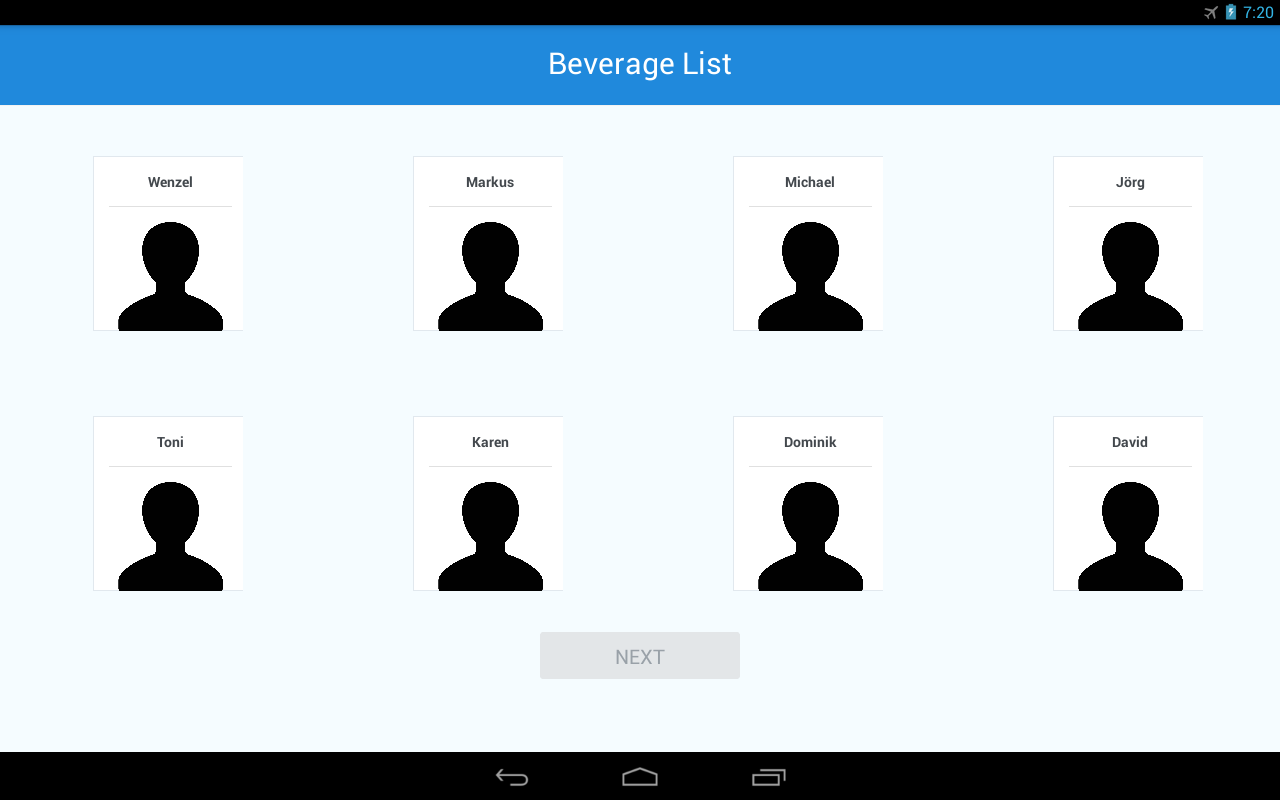
\includegraphics[width=.9\columnwidth]{./Abbildungen/Kapitel_03/emps1.png}
	\caption{Mitarbeiter Page: kein Mitarbeiter ausgewählt}
	\label{img:emps1}
\end{figure}

\begin{figure}[th!]
	\centering
	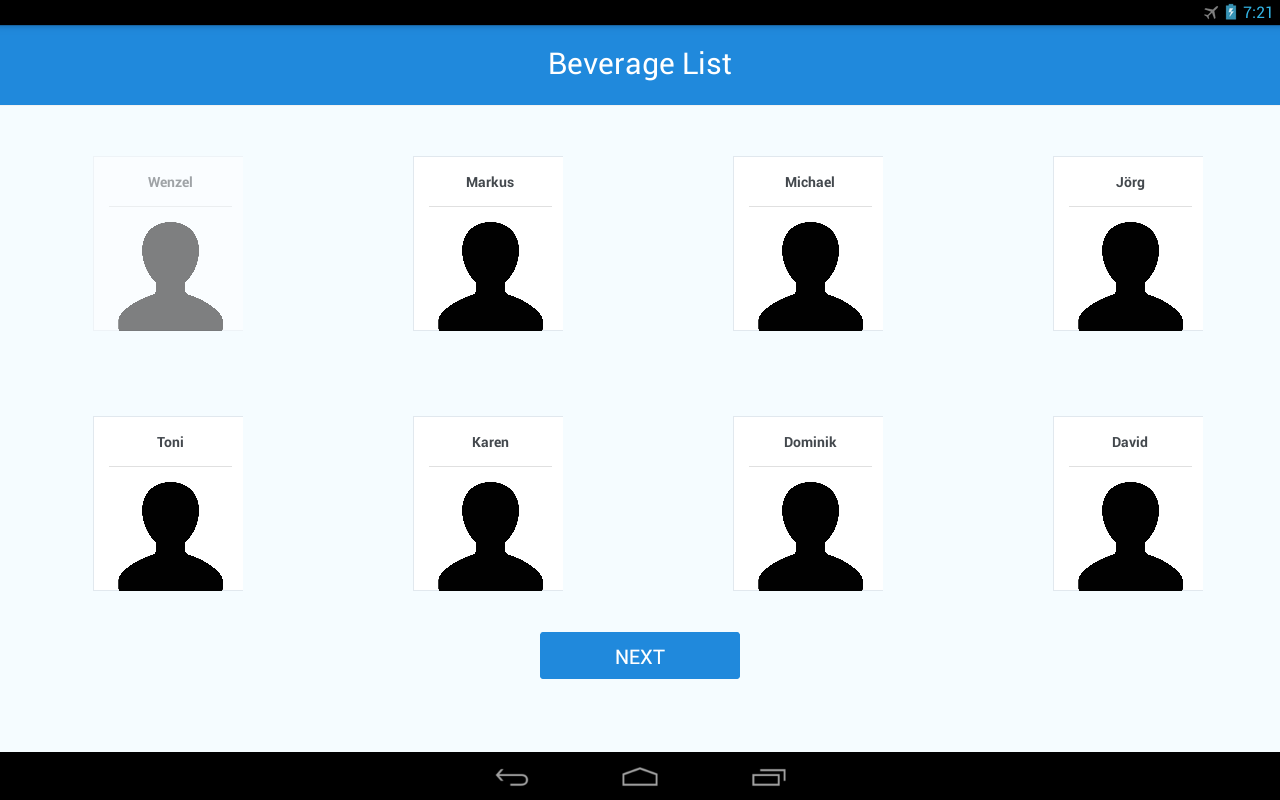
\includegraphics[width=.9\columnwidth]{./Abbildungen/Kapitel_03/emps2.png}
	\caption{Mitarbeiter Page: Mitarbeiter ausgewählt}
	\label{img:emps2}
\end{figure}

Hier kann der User seinen Avatar selektieren und deselektieren. Ist ein Avatar ausgewählt wird der \quotes{NEXT} Button aktiviert (vgl. Abbildung \ref{img:emps2}) und durch dessen Betätigung gelangt der User zur nächsten Seite: 

\begin{figure}[th!]
	\centering
	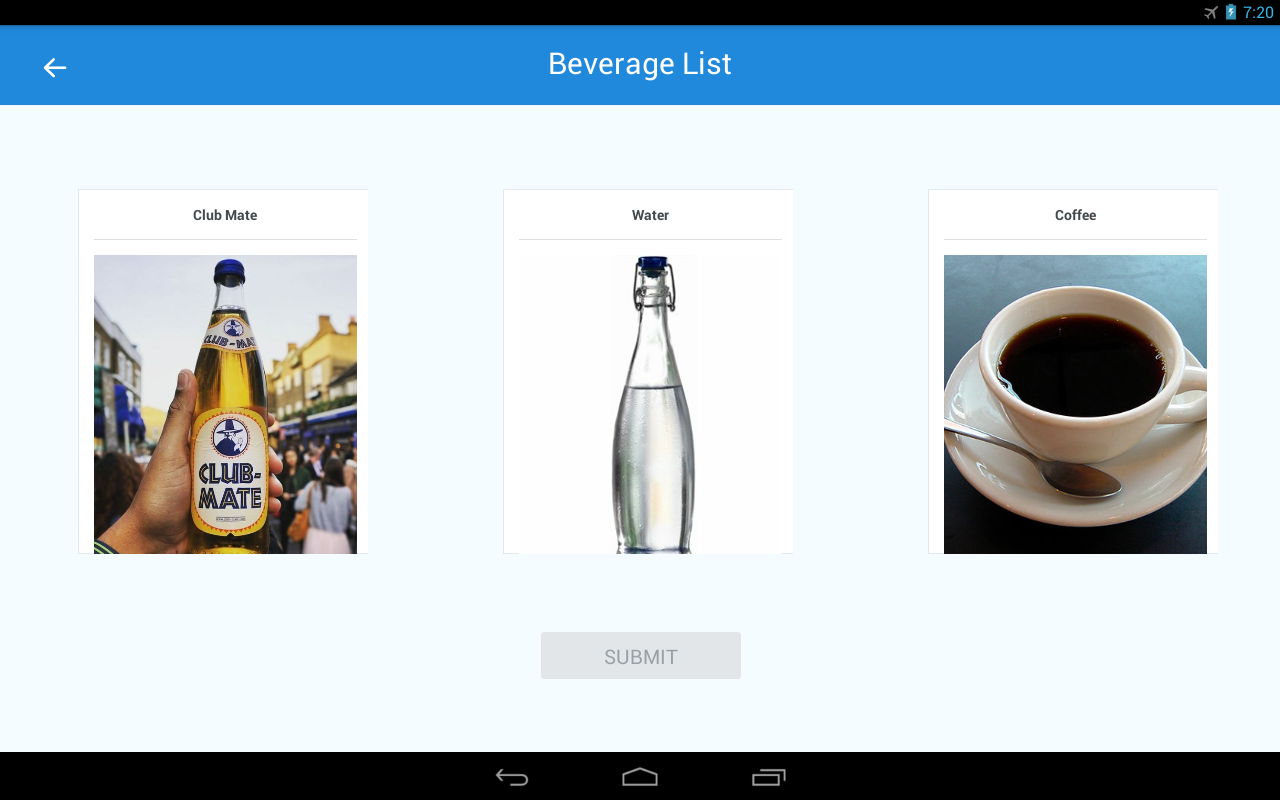
\includegraphics[width=.9\columnwidth]{./Abbildungen/Kapitel_03/drinks1.png}
	\caption{Drinks Page: kein Getränk ausgewählt}
	\label{img:drinks1}
\end{figure}

Hier besteht eine Auswahl aus folgenden Getränken: Club Mate, Wasser und Kaffee. 
Ausgewählt kann jedoch immer nur eines werden (vgl. Abbildung \ref{img:drinks2}).
Das Prinzip der Selektion und Deselektion ist identisch mit dem der vorherigen Seite. So wird der \quotes{SUBMIT} Button aktiv, sobald ein Getränk ausgewählt ist und inaktiv wenn das Getränk wieder deselektiert wird (vgl. Abbildung \ref{img:drinks1}).\\

\begin{figure}[th!]
	\centering
	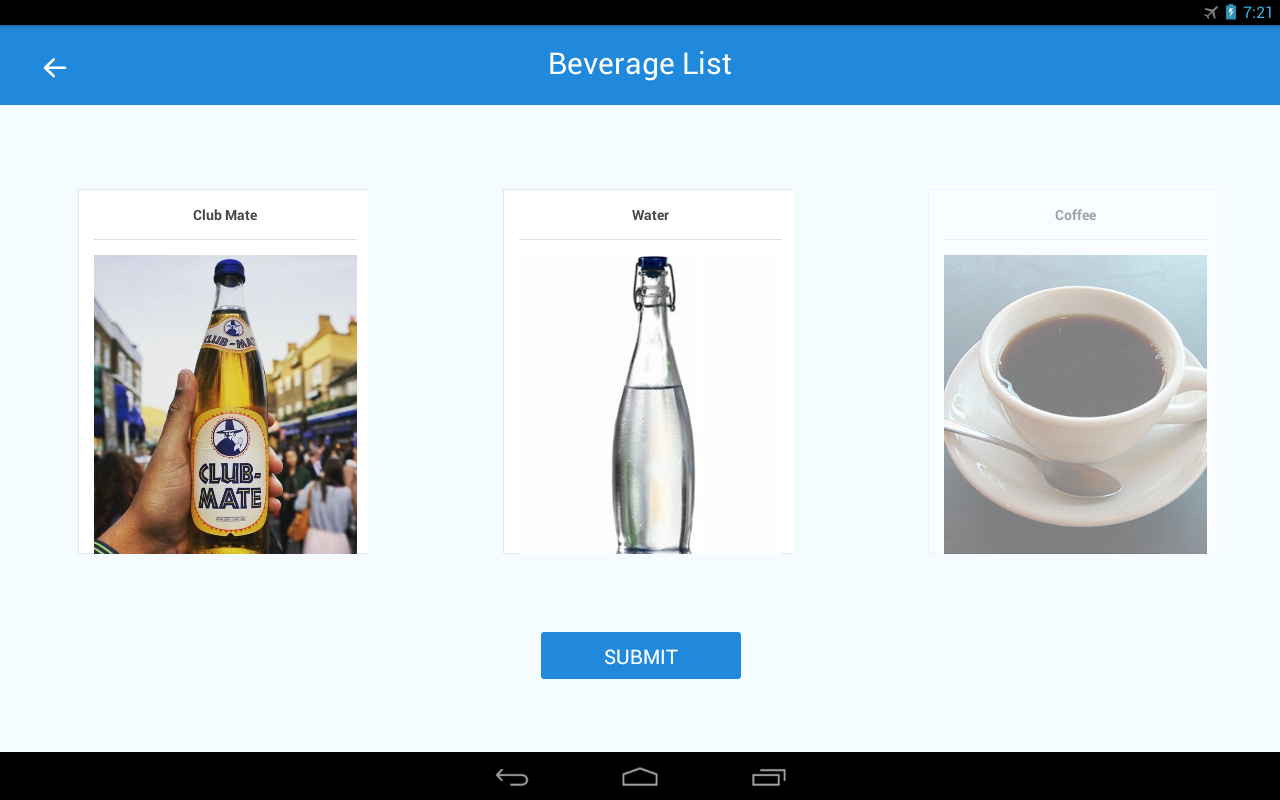
\includegraphics[width=.9\columnwidth]{./Abbildungen/Kapitel_03/drinks2.png}
	\caption{Drinks Page: Getränk ausgewählt}
	\label{img:drinks2}
\end{figure}

Wird schließlich der \quotes{SUBMIT} Button gedrückt und die Transaktion als erfolgreich bestätigt erscheint folgendes Overlay:

\begin{figure}[th!]
	\centering
	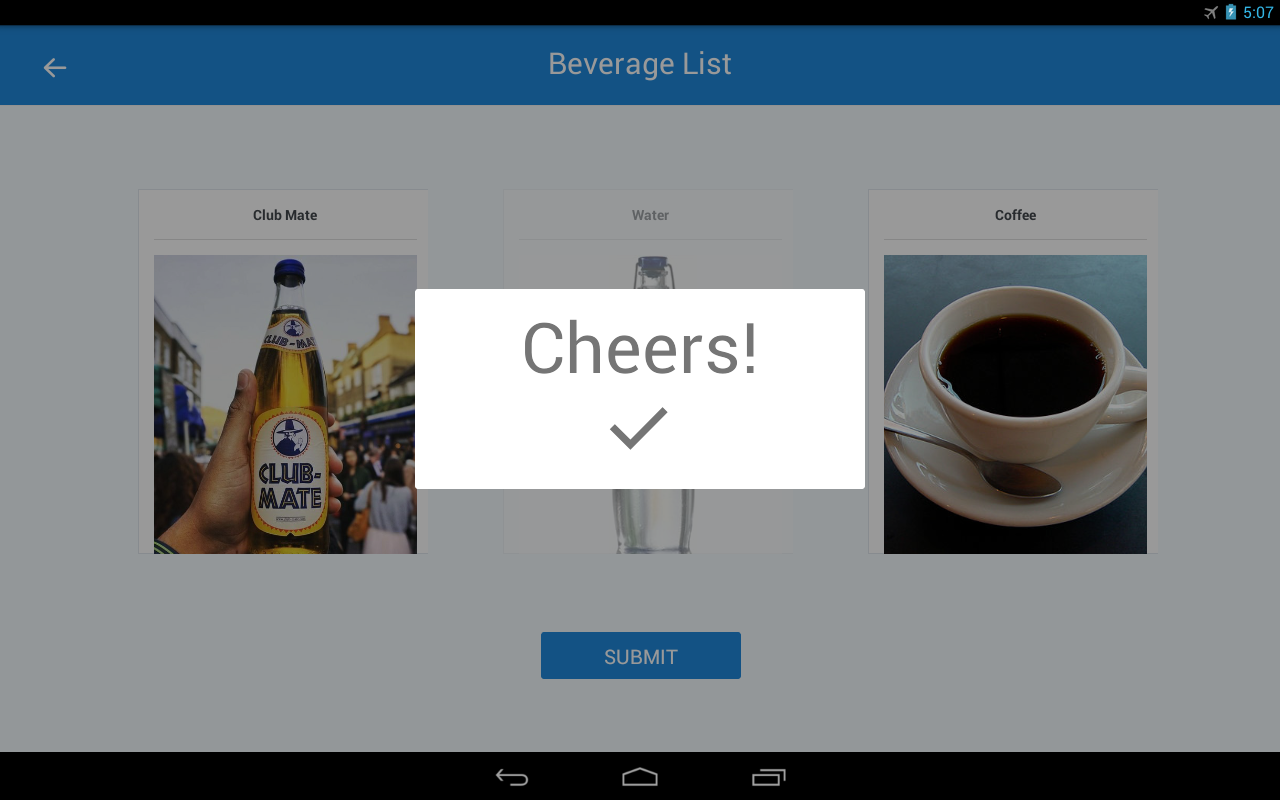
\includegraphics[width=.9\columnwidth]{./Abbildungen/Kapitel_03/cheers.png}
	\caption{}
	\label{img:drinks2}
\end{figure}

Nach 4 Sekunden wird dieses Overlay wieder ausgeblendet und automatisch zur Startseite (vgl. Abbildung \ref{img:emps1}) navigiert, wodurch der Workflow von neuem startet.\\\\
Aufgrund der Tatsache, dass die Verbindung zum Uni-Netzwerk (eduroam) nur über einen Workaround hergestellt werden konnte, bei dem die Verbindung zum Netzwerk trotzdessen nach einer unbestimmten Zeit immer wieder abgebrochen ist, wurde eine weitere Komponente entwickelt.

\begin{figure}[th!]
	\centering
	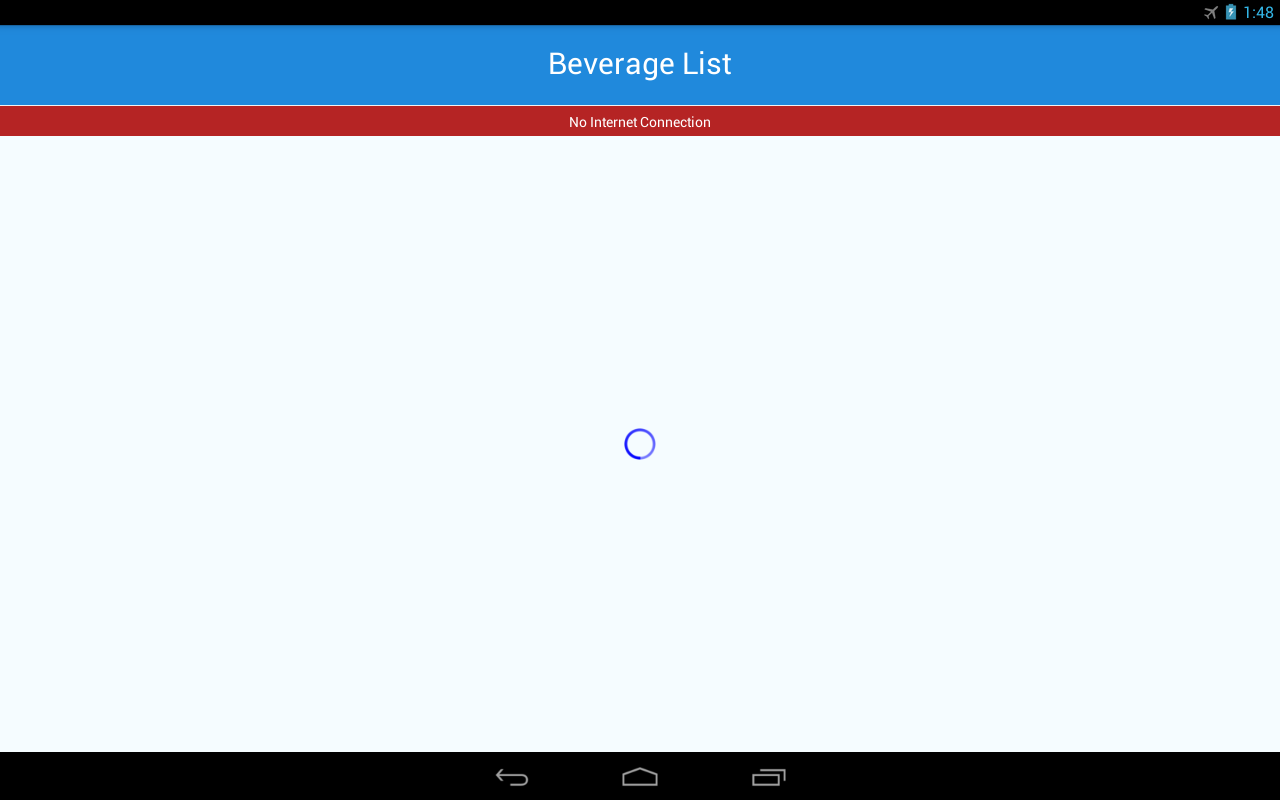
\includegraphics[width=.9\columnwidth]{./Abbildungen/Kapitel_03/noconnection.png}
	\caption{}
	\label{img:drinks2}
\end{figure}

Diese wird sofort eingeblendet sobald die Verbindung zum Internet unterbrochen ist, allerdings nur wenn sich der User auf der Startseite befindet. Wird die Seite mit den Getränken angezeigt, so wird dem User die Möglichkeit gegeben seine Transaktion abzuschließen. Da in diesem Moment jedoch keine Verbindung zur Blockchain hergestellt werden kann, werden die Transaktionsdaten zwischengespeichert und diese durchgeführt sobald wieder eine Verbindung zum Netzwerk besteht (vgl. Kap. \ref{subsec:internalFlow}).
Die Loading Animation sowie das \quotes{No Internet Connection} Label werden wieder ausgeblendet sobald die App eine erneute Verbindung zum Uni-Netzwerk detektiert.

\subsection{Internal Workflow}
\label{subsec:internalFlow}
Basierend auf der Problematik eines unerwarteten Verbindungsabbruch und dem einhergehenden Verlust von essentiellen Lerndaten, wird im folgenden der implementierte Algorithmus geschildert, der dieser Komplikation entgegenwirkt. 

\begin{legal}
	\item Initialisierungsphase:
	\begin{legal}
		\item \quotes{GET} Smart Contract Daten von Fileserver
		\item Initialisierung Web3.js
		\item Wiederhole für jedes Transaktionsfile:
		\begin{legal}
			\item Transaktion durchführen
			\item bei \quotes{Success} Transaktiondatei löschen
		\end{legal}
	\end{legal}
	\item Warten auf Usereingabe:
	\begin{legal}
		\item User ausgewählt $\rightarrow$ Ethereum-Adresse
		\item Getränk ausgewählt $\rightarrow$ Getränk
		\item Submit $\rightarrow$ (Getränk \& Ethereum-Adresse)
	\end{legal}
	\item Wiederhole für jedes User-Transaktionsfile:
	\begin{legal}
		\item Transaktion durchführen
		\item bei \quotes{Success} Transaktiondatei löschen
	\end{legal}
	\item Generierung Transaktionsdaten:
	\begin{itemize}
		\item Gas Estimate
		\item Datum (inkl. Zeit)
		\item Wochentag
		\item Ethereum-Adresse \& Getränk aus 2.3
	\end{itemize}
	\item Transaktion starten:
	\begin{legal}
		\item Erstellung der Transaktiondatei
		\item Transaktion durchführen
		\item bei \quotes{Success} Transaktiondatei löschen
		\item gehe zu 1.
	\end{legal} 	
\end{legal}

Der interne Workflow beginnt mit der Initialisierungsphase, dabei werden zuerst die Smart Contract Files vom Fileserver runtergeladen und mit den beinhaltenden Daten das Web3.js Modul initialisiert. Damit steht Verbindung und die Kommunikation mit den Smart Contracts und es wird im Anschluss über alle vorhandenen Transaktion Files iteriert. Dabei wird zuerst der CoffeeCoin Contract und dann der Beveragelist Contract aufgerufen. Wenn beide ihre Transaktionen bestätigt haben, wird die Datei gelöscht, andernfalls bleibt diese bestehen. Dies geschieht noch bevor der User das Interface zu Gesicht bekommt.\\\\
Nachdem 1. abgeschlossen ist wird auf die Eingabe des Users gewartet. Wählt dieser einen Avatar aus klickt \quotes{NEXT} wird seine hinterlegte Ethereum-Adresse temporär gespeichert. Wird dann im Anschluss ein Getränk selektiert und \quotes{SUBMIT} gedrückt, werden die Ethereum-Adresse und das Getränk an das interne Blockchain-Modul weitergereicht und die Transaktion gestartet. \\\\
Dabei wird erneut über die Transaktionsdaten iteriert, allerdings nur über die des Users. Damit soll stets die richtige Reihenfolge der getrunkenen Getränke sichergestellt werden, da dies ansonsten auf Seiten des Q-Learning Algorithmus zu falschen Lerneffekten führen würde.\\\\
Daraufhin kann mit der Generierung der fehlenden Transaktionsdaten angefangen werde. Es wird zuerst ein \quotes{Gas Estimate} für beide Smart Contract Transaktionen durchgeführt. Ein \quotes{Gas Estimate} ist, wie der Name bereits impliziert, eine grobe Schätzung wie viel Gas beim Funktionsaufruf eines Smart Contracts benötigt wird. Abschließend werden das Datum (inkl. Zeit in Sekunden) und der Wochentag ermittelt und alle benötigten Daten an die jeweiligen Smart Contract Funktionsaufrufe übergeben. Im Falle des Smart Contracts Beveragelist: \textit{Gas-Estimate, Datum, Wochentag, Ethereum-Adresse, Getränk}.
Bei CoffeeCoin wird anhand des Getränks die entsprechende Smart Contract Funktion ausgewählt und lediglich das \textit{Gas-Estimate} und die \textit{Ethereum-Adresse} des Users übergeben.\\\\
Bevor jedoch beide Transaktionen durchgeführt werden, wird ein Transaktionsfile mit dem Namen \quotes{<<ethereum-adresse>>-<<datum>>.json} und den Daten \textit{Datum, Wochentag, Ethereum-Adresse, Getränk} gespeichert. Sogleich werden beide Funktionsaufrufe getätigt und bei erfolgreicher Bestätigung beider Transaktionen wird das gerade erstellte File wieder gelöscht. Somit soll sichergestellt werden, dass keine Transaktionen aufgrund von Verbindungsabbrüchen verloren gehen. \\\\
Anschließend erfolgt eine \quotes{Pseudo-Reload} der App und der Ablauf beginnt wieder bei 1.